% !TEX program = pdflatex
% Credit, capital and buybacks: can Q/Y rise without the dividend channel? 18 Nov 2026.
% Numbers: data/values.tex (\val{key}), written by scripts/build.py; figures: figures/ (drawn by build.py).
% Preamble and colors as in Logistics/Discussion_note/29_11_16/slides/main.tex.
\documentclass[aspectratio=169,10pt,t]{beamer}
\usepackage[T1]{fontenc}
\usepackage[utf8]{inputenc}
\usepackage{lmodern,amsmath,amssymb,booktabs,graphicx,array,xcolor}
\usetheme{default}
\setbeamertemplate{navigation symbols}{}
\setbeamertemplate{footline}{\hfill\textcolor{muted}{\scriptsize\insertframenumber}\hspace{0.4cm}\vspace{0.25cm}}
\setbeamertemplate{itemize items}[circle]
\setbeamertemplate{frametitle}{\vspace{0.3cm}\textbf{\large\insertframetitle}\ifx\insertframesubtitle\empty\else\\[-0.05cm]{\small\textcolor{inksec}{\insertframesubtitle}}\fi\vspace{0.05cm}}
\definecolor{ink}{HTML}{0B0B0B}\definecolor{inksec}{HTML}{52514E}\definecolor{muted}{HTML}{898781}
\definecolor{dataC}{HTML}{2A78D6}\definecolor{dataD}{HTML}{104281}\definecolor{modelC}{HTML}{EB6834}\definecolor{washc}{HTML}{F0EFEC}
\setbeamercolor{normal text}{fg=ink,bg=white}\setbeamercolor{structure}{fg=dataD}\setbeamercolor{frametitle}{fg=ink}
\setbeamercolor{block title}{fg=white,bg=dataD}\setbeamercolor{block body}{fg=ink,bg=washc}
\setlength{\leftmargini}{1.1em}
\newcommand{\val}[1]{\csname v:#1\endcsname}
\expandafter\def\csname v:vintage_fcf_diff\endcsname{0.00}
\expandafter\def\csname v:vintage_q_diff\endcsname{0.00}
\expandafter\def\csname v:latest_q\endcsname{2026Q2}
\expandafter\def\csname v:lat_QY\endcsname{546}
\expandafter\def\csname v:lat_DEBTY\endcsname{97.0}
\expandafter\def\csname v:lat_KY\endcsname{203}
\expandafter\def\csname v:lat_PCY\endcsname{6.93}
\expandafter\def\csname v:lat_EQY\endcsname{586}
\expandafter\def\csname v:lat_q\endcsname{2.70}
\expandafter\def\csname v:lat_NB_ttm\endcsname{826}
\expandafter\def\csname v:lat_NBY\endcsname{5.10}
\expandafter\def\csname v:lat_BUYY\endcsname{-0.19}
\expandafter\def\csname v:lat_NCFY\endcsname{3.82}
\expandafter\def\csname v:QY1990\endcsname{143}
\expandafter\def\csname v:EQY1990\endcsname{107}
\expandafter\def\csname v:DEBTY1990\endcsname{82.7}
\expandafter\def\csname v:BONDSY1990\endcsname{39.7}
\expandafter\def\csname v:LOANSY1990\endcsname{43.0}
\expandafter\def\csname v:PCY1990\endcsname{0.00}
\expandafter\def\csname v:KY1990\endcsname{210}
\expandafter\def\csname v:REY1990\endcsname{106}
\expandafter\def\csname v:EQPY1990\endcsname{57.5}
\expandafter\def\csname v:IPPY1990\endcsname{15.4}
\expandafter\def\csname v:INVY1990\endcsname{28.8}
\expandafter\def\csname v:FCFY1990\endcsname{7.12}
\expandafter\def\csname v:DEQY1990\endcsname{5.74}
\expandafter\def\csname v:DIVY1990\endcsname{3.74}
\expandafter\def\csname v:BUYY1990\endcsname{2.00}
\expandafter\def\csname v:NBY1990\endcsname{4.23}
\expandafter\def\csname v:NCFY1990\endcsname{4.22}
\expandafter\def\csname v:q1990\endcsname{0.68}
\expandafter\def\csname v:Y_tn1990\endcsname{3.16}
\expandafter\def\csname v:Q_tn1990\endcsname{4.53}
\expandafter\def\csname v:DEBT_tn1990\endcsname{2.61}
\expandafter\def\csname v:QY2000\endcsname{258}
\expandafter\def\csname v:EQY2000\endcsname{280}
\expandafter\def\csname v:DEBTY2000\endcsname{87.6}
\expandafter\def\csname v:BONDSY2000\endcsname{49.9}
\expandafter\def\csname v:LOANSY2000\endcsname{37.7}
\expandafter\def\csname v:PCY2000\endcsname{0.00}
\expandafter\def\csname v:KY2000\endcsname{198}
\expandafter\def\csname v:REY2000\endcsname{98.4}
\expandafter\def\csname v:EQPY2000\endcsname{52.5}
\expandafter\def\csname v:IPPY2000\endcsname{19.7}
\expandafter\def\csname v:INVY2000\endcsname{24.3}
\expandafter\def\csname v:FCFY2000\endcsname{2.68}
\expandafter\def\csname v:DEQY2000\endcsname{5.21}
\expandafter\def\csname v:DIVY2000\endcsname{4.56}
\expandafter\def\csname v:BUYY2000\endcsname{0.65}
\expandafter\def\csname v:NBY2000\endcsname{6.37}
\expandafter\def\csname v:NCFY2000\endcsname{7.50}
\expandafter\def\csname v:q2000\endcsname{1.30}
\expandafter\def\csname v:Y_tn2000\endcsname{5.51}
\expandafter\def\csname v:Q_tn2000\endcsname{14.2}
\expandafter\def\csname v:DEBT_tn2000\endcsname{4.83}
\expandafter\def\csname v:QY2007\endcsname{235}
\expandafter\def\csname v:EQY2007\endcsname{269}
\expandafter\def\csname v:DEBTY2007\endcsname{91.5}
\expandafter\def\csname v:BONDSY2007\endcsname{47.8}
\expandafter\def\csname v:LOANSY2007\endcsname{43.8}
\expandafter\def\csname v:PCY2007\endcsname{0.00}
\expandafter\def\csname v:KY2007\endcsname{241}
\expandafter\def\csname v:REY2007\endcsname{138}
\expandafter\def\csname v:EQPY2007\endcsname{50.2}
\expandafter\def\csname v:IPPY2007\endcsname{21.4}
\expandafter\def\csname v:INVY2007\endcsname{25.6}
\expandafter\def\csname v:FCFY2007\endcsname{8.64}
\expandafter\def\csname v:DEQY2007\endcsname{14.1}
\expandafter\def\csname v:DIVY2007\endcsname{6.66}
\expandafter\def\csname v:BUYY2007\endcsname{7.45}
\expandafter\def\csname v:NBY2007\endcsname{9.46}
\expandafter\def\csname v:NCFY2007\endcsname{5.06}
\expandafter\def\csname v:q2007\endcsname{0.98}
\expandafter\def\csname v:Y_tn2007\endcsname{7.26}
\expandafter\def\csname v:Q_tn2007\endcsname{17.1}
\expandafter\def\csname v:DEBT_tn2007\endcsname{6.64}
\expandafter\def\csname v:QY2009\endcsname{224}
\expandafter\def\csname v:EQY2009\endcsname{229}
\expandafter\def\csname v:DEBTY2009\endcsname{93.8}
\expandafter\def\csname v:BONDSY2009\endcsname{55.6}
\expandafter\def\csname v:LOANSY2009\endcsname{38.2}
\expandafter\def\csname v:PCY2009\endcsname{0.00}
\expandafter\def\csname v:KY2009\endcsname{202}
\expandafter\def\csname v:REY2009\endcsname{92.7}
\expandafter\def\csname v:EQPY2009\endcsname{54.5}
\expandafter\def\csname v:IPPY2009\endcsname{24.2}
\expandafter\def\csname v:INVY2009\endcsname{24.7}
\expandafter\def\csname v:FCFY2009\endcsname{13.9}
\expandafter\def\csname v:DEQY2009\endcsname{6.62}
\expandafter\def\csname v:DIVY2009\endcsname{5.33}
\expandafter\def\csname v:BUYY2009\endcsname{1.29}
\expandafter\def\csname v:NBY2009\endcsname{-5.17}
\expandafter\def\csname v:NCFY2009\endcsname{-0.53}
\expandafter\def\csname v:q2009\endcsname{1.11}
\expandafter\def\csname v:Y_tn2009\endcsname{6.90}
\expandafter\def\csname v:Q_tn2009\endcsname{15.5}
\expandafter\def\csname v:DEBT_tn2009\endcsname{6.48}
\expandafter\def\csname v:QY2011\endcsname{261}
\expandafter\def\csname v:EQY2011\endcsname{235}
\expandafter\def\csname v:DEBTY2011\endcsname{87.6}
\expandafter\def\csname v:BONDSY2011\endcsname{56.2}
\expandafter\def\csname v:LOANSY2011\endcsname{31.5}
\expandafter\def\csname v:PCY2011\endcsname{0.00}
\expandafter\def\csname v:KY2011\endcsname{209}
\expandafter\def\csname v:REY2011\endcsname{101}
\expandafter\def\csname v:EQPY2011\endcsname{52.5}
\expandafter\def\csname v:IPPY2011\endcsname{23.9}
\expandafter\def\csname v:INVY2011\endcsname{26.1}
\expandafter\def\csname v:FCFY2011\endcsname{12.8}
\expandafter\def\csname v:DEQY2011\endcsname{10.5}
\expandafter\def\csname v:DIVY2011\endcsname{6.02}
\expandafter\def\csname v:BUYY2011\endcsname{4.51}
\expandafter\def\csname v:NBY2011\endcsname{4.47}
\expandafter\def\csname v:NCFY2011\endcsname{3.37}
\expandafter\def\csname v:q2011\endcsname{1.25}
\expandafter\def\csname v:Y_tn2011\endcsname{7.66}
\expandafter\def\csname v:Q_tn2011\endcsname{20.0}
\expandafter\def\csname v:DEBT_tn2011\endcsname{6.71}
\expandafter\def\csname v:QY2019\endcsname{397}
\expandafter\def\csname v:EQY2019\endcsname{394}
\expandafter\def\csname v:DEBTY2019\endcsname{103}
\expandafter\def\csname v:BONDSY2019\endcsname{65.0}
\expandafter\def\csname v:LOANSY2019\endcsname{38.4}
\expandafter\def\csname v:PCY2019\endcsname{2.94}
\expandafter\def\csname v:KY2019\endcsname{228}
\expandafter\def\csname v:REY2019\endcsname{121}
\expandafter\def\csname v:EQPY2019\endcsname{49.3}
\expandafter\def\csname v:IPPY2019\endcsname{26.2}
\expandafter\def\csname v:INVY2019\endcsname{24.5}
\expandafter\def\csname v:FCFY2019\endcsname{10.5}
\expandafter\def\csname v:DEQY2019\endcsname{9.33}
\expandafter\def\csname v:DIVY2019\endcsname{6.18}
\expandafter\def\csname v:BUYY2019\endcsname{3.15}
\expandafter\def\csname v:NBY2019\endcsname{6.43}
\expandafter\def\csname v:NCFY2019\endcsname{4.94}
\expandafter\def\csname v:q2019\endcsname{1.74}
\expandafter\def\csname v:Y_tn2019\endcsname{10.8}
\expandafter\def\csname v:Q_tn2019\endcsname{42.9}
\expandafter\def\csname v:DEBT_tn2019\endcsname{11.2}
\expandafter\def\csname v:QY2021\endcsname{492}
\expandafter\def\csname v:EQY2021\endcsname{519}
\expandafter\def\csname v:DEBTY2021\endcsname{109}
\expandafter\def\csname v:BONDSY2021\endcsname{66.4}
\expandafter\def\csname v:LOANSY2021\endcsname{42.8}
\expandafter\def\csname v:PCY2021\endcsname{4.32}
\expandafter\def\csname v:KY2021\endcsname{237}
\expandafter\def\csname v:REY2021\endcsname{128}
\expandafter\def\csname v:EQPY2021\endcsname{48.3}
\expandafter\def\csname v:IPPY2021\endcsname{27.6}
\expandafter\def\csname v:INVY2021\endcsname{26.3}
\expandafter\def\csname v:FCFY2021\endcsname{14.6}
\expandafter\def\csname v:DEQY2021\endcsname{10.0}
\expandafter\def\csname v:DIVY2021\endcsname{9.59}
\expandafter\def\csname v:BUYY2021\endcsname{0.45}
\expandafter\def\csname v:NBY2021\endcsname{5.72}
\expandafter\def\csname v:NCFY2021\endcsname{3.74}
\expandafter\def\csname v:q2021\endcsname{2.07}
\expandafter\def\csname v:Y_tn2021\endcsname{12.1}
\expandafter\def\csname v:Q_tn2021\endcsname{59.4}
\expandafter\def\csname v:DEBT_tn2021\endcsname{13.2}
\expandafter\def\csname v:QY2025\endcsname{497}
\expandafter\def\csname v:EQY2025\endcsname{532}
\expandafter\def\csname v:DEBTY2025\endcsname{97.2}
\expandafter\def\csname v:BONDSY2025\endcsname{57.3}
\expandafter\def\csname v:LOANSY2025\endcsname{39.9}
\expandafter\def\csname v:PCY2025\endcsname{6.97}
\expandafter\def\csname v:KY2025\endcsname{202}
\expandafter\def\csname v:REY2025\endcsname{96.2}
\expandafter\def\csname v:EQPY2025\endcsname{46.2}
\expandafter\def\csname v:IPPY2025\endcsname{29.4}
\expandafter\def\csname v:INVY2025\endcsname{23.7}
\expandafter\def\csname v:FCFY2025\endcsname{11.8}
\expandafter\def\csname v:DEQY2025\endcsname{11.2}
\expandafter\def\csname v:DIVY2025\endcsname{8.98}
\expandafter\def\csname v:BUYY2025\endcsname{2.23}
\expandafter\def\csname v:NBY2025\endcsname{4.56}
\expandafter\def\csname v:NCFY2025\endcsname{4.17}
\expandafter\def\csname v:q2025\endcsname{2.45}
\expandafter\def\csname v:Y_tn2025\endcsname{15.6}
\expandafter\def\csname v:Q_tn2025\endcsname{77.5}
\expandafter\def\csname v:DEBT_tn2025\endcsname{15.2}
\expandafter\def\csname v:nfc_share_q2025\endcsname{92.7}
\expandafter\def\csname v:PC_tn2025\endcsname{1.09}
\expandafter\def\csname v:dec2009_dQY_pp\endcsname{272}
\expandafter\def\csname v:dec2009_dEY_pp\endcsname{263}
\expandafter\def\csname v:dec2009_dFDIY_pp\endcsname{39.9}
\expandafter\def\csname v:dec2009_dDEBTY_pp\endcsname{3.40}
\expandafter\def\csname v:dec2009_dOTHERY_pp\endcsname{-34.4}
\expandafter\def\csname v:dec2009_sh_E\endcsname{96.7}
\expandafter\def\csname v:dec2009_sh_FDI\endcsname{14.7}
\expandafter\def\csname v:dec2009_sh_DEBT\endcsname{1.25}
\expandafter\def\csname v:dec2009_sh_OTHER\endcsname{-12.6}
\expandafter\def\csname v:dec2009_dlogQY\endcsname{0.79}
\expandafter\def\csname v:dec2009_dlog_q\endcsname{0.79}
\expandafter\def\csname v:dec2009_dlog_KY\endcsname{0.00}
\expandafter\def\csname v:dec2009_sh_q\endcsname{99.9}
\expandafter\def\csname v:dec2009_sh_KY\endcsname{0.07}
\expandafter\def\csname v:dec2011_dQY_pp\endcsname{236}
\expandafter\def\csname v:dec2011_dEY_pp\endcsname{258}
\expandafter\def\csname v:dec2011_dFDIY_pp\endcsname{39.1}
\expandafter\def\csname v:dec2011_dDEBTY_pp\endcsname{9.58}
\expandafter\def\csname v:dec2011_dOTHERY_pp\endcsname{-70.9}
\expandafter\def\csname v:dec2011_sh_E\endcsname{109}
\expandafter\def\csname v:dec2011_sh_FDI\endcsname{16.6}
\expandafter\def\csname v:dec2011_sh_DEBT\endcsname{4.07}
\expandafter\def\csname v:dec2011_sh_OTHER\endcsname{-30.1}
\expandafter\def\csname v:dec2011_dlogQY\endcsname{0.64}
\expandafter\def\csname v:dec2011_dlog_q\endcsname{0.68}
\expandafter\def\csname v:dec2011_dlog_KY\endcsname{-0.03}
\expandafter\def\csname v:dec2011_sh_q\endcsname{105}
\expandafter\def\csname v:dec2011_sh_KY\endcsname{-5.28}
\expandafter\def\csname v:avg_pre_NB\endcsname{4.29}
\expandafter\def\csname v:avg_pre_BUY\endcsname{1.65}
\expandafter\def\csname v:avg_pre_DIV\endcsname{4.65}
\expandafter\def\csname v:avg_pre_DEQ\endcsname{6.30}
\expandafter\def\csname v:avg_pre_NCF\endcsname{5.01}
\expandafter\def\csname v:avg_pre_CAPX\endcsname{18.5}
\expandafter\def\csname v:avg_pre_FCF\endcsname{7.00}
\expandafter\def\csname v:avg_pre_NAFA\endcsname{9.44}
\expandafter\def\csname v:avg_pre_INT\endcsname{3.40}
\expandafter\def\csname v:avg_post_NB\endcsname{4.36}
\expandafter\def\csname v:avg_post_BUY\endcsname{3.25}
\expandafter\def\csname v:avg_post_DIV\endcsname{7.35}
\expandafter\def\csname v:avg_post_DEQ\endcsname{10.6}
\expandafter\def\csname v:avg_post_NCF\endcsname{4.22}
\expandafter\def\csname v:avg_post_CAPX\endcsname{19.7}
\expandafter\def\csname v:avg_post_FCF\endcsname{11.8}
\expandafter\def\csname v:avg_post_NAFA\endcsname{8.70}
\expandafter\def\csname v:avg_post_INT\endcsname{3.14}
\expandafter\def\csname v:avg_postB_NB\endcsname{5.34}
\expandafter\def\csname v:avg_postB_BUY\endcsname{3.44}
\expandafter\def\csname v:avg_postB_DIV\endcsname{7.62}
\expandafter\def\csname v:avg_postB_DEQ\endcsname{11.1}
\expandafter\def\csname v:avg_postB_NCF\endcsname{4.66}
\expandafter\def\csname v:avg_postB_CAPX\endcsname{20.0}
\expandafter\def\csname v:avg_postB_FCF\endcsname{11.5}
\expandafter\def\csname v:avg_postB_NAFA\endcsname{9.12}
\expandafter\def\csname v:avg_postB_INT\endcsname{2.99}
\expandafter\def\csname v:cum_NB\endcsname{8.09}
\expandafter\def\csname v:cum_BUY\endcsname{5.72}
\expandafter\def\csname v:cum_DIV\endcsname{13.6}
\expandafter\def\csname v:cum_NCF\endcsname{7.76}
\expandafter\def\csname v:cum_FCF\endcsname{20.8}
\expandafter\def\csname v:cum_DEQ\endcsname{19.4}
\expandafter\def\csname v:cum_dDEBT\endcsname{8.69}
\expandafter\def\csname v:cum_dQ\endcsname{62.0}
\expandafter\def\csname v:cum_dEQ\endcsname{67.2}
\expandafter\def\csname v:cum_dK\endcsname{17.6}
\expandafter\def\csname v:debt_min_post\endcsname{87.5}
\expandafter\def\csname v:debt_max_post\endcsname{117}
\expandafter\def\csname v:debt_max_post_year\endcsname{2,020}
\expandafter\def\csname v:K_min_post\endcsname{202}
\expandafter\def\csname v:K_max_post\endcsname{242}
\expandafter\def\csname v:rob_fcfa_yield_start\endcsname{6.20}
\expandafter\def\csname v:rob_fcfa_yield_end\endcsname{2.38}
\expandafter\def\csname v:rob_fcfa_dlog_QD\endcsname{0.96}
\expandafter\def\csname v:rob_fcfa_dlog_QY\endcsname{0.79}
\expandafter\def\csname v:rob_fcfa_dlog_DY\endcsname{-0.16}
\expandafter\def\csname v:rob_fcfa_share_QY\endcsname{83.0}
\expandafter\def\csname v:rob_deqa_yield_start\endcsname{2.89}
\expandafter\def\csname v:rob_deqa_yield_end\endcsname{2.11}
\expandafter\def\csname v:rob_deqa_dlog_QD\endcsname{0.32}
\expandafter\def\csname v:rob_deqa_dlog_QY\endcsname{0.84}
\expandafter\def\csname v:rob_deqa_dlog_DY\endcsname{0.53}
\expandafter\def\csname v:rob_deqa_share_QY\endcsname{266}
\expandafter\def\csname v:rob_diva_yield_start\endcsname{2.33}
\expandafter\def\csname v:rob_diva_yield_end\endcsname{1.69}
\expandafter\def\csname v:rob_diva_dlog_QD\endcsname{0.32}
\expandafter\def\csname v:rob_diva_dlog_QY\endcsname{0.84}
\expandafter\def\csname v:rob_diva_dlog_DY\endcsname{0.52}
\expandafter\def\csname v:rob_diva_share_QY\endcsname{262}
\expandafter\def\csname v:rob_fcfb_yield_start\endcsname{4.88}
\expandafter\def\csname v:rob_fcfb_yield_end\endcsname{2.38}
\expandafter\def\csname v:rob_fcfb_dlog_QD\endcsname{0.72}
\expandafter\def\csname v:rob_fcfb_dlog_QY\endcsname{0.64}
\expandafter\def\csname v:rob_fcfb_dlog_DY\endcsname{-0.07}
\expandafter\def\csname v:rob_fcfb_share_QY\endcsname{89.6}
\expandafter\def\csname v:rob_deqb_yield_start\endcsname{4.48}
\expandafter\def\csname v:rob_deqb_yield_end\endcsname{2.11}
\expandafter\def\csname v:rob_deqb_dlog_QD\endcsname{0.75}
\expandafter\def\csname v:rob_deqb_dlog_QY\endcsname{0.82}
\expandafter\def\csname v:rob_deqb_dlog_DY\endcsname{0.06}
\expandafter\def\csname v:rob_deqb_share_QY\endcsname{108}
\expandafter\def\csname v:rob_divb_yield_start\endcsname{2.56}
\expandafter\def\csname v:rob_divb_yield_end\endcsname{1.69}
\expandafter\def\csname v:rob_divb_dlog_QD\endcsname{0.42}
\expandafter\def\csname v:rob_divb_dlog_QY\endcsname{0.82}
\expandafter\def\csname v:rob_divb_dlog_DY\endcsname{0.40}
\expandafter\def\csname v:rob_divb_share_QY\endcsname{196}
\expandafter\def\csname v:rob_fcfc_yield_start\endcsname{5.36}
\expandafter\def\csname v:rob_fcfc_yield_end\endcsname{2.58}
\expandafter\def\csname v:rob_fcfc_dlog_QD\endcsname{0.73}
\expandafter\def\csname v:rob_fcfc_dlog_QY\endcsname{0.61}
\expandafter\def\csname v:rob_fcfc_dlog_DY\endcsname{-0.12}
\expandafter\def\csname v:rob_fcfc_share_QY\endcsname{83.5}
\expandafter\def\csname v:rob_deqc_yield_start\endcsname{3.49}
\expandafter\def\csname v:rob_deqc_yield_end\endcsname{2.65}
\expandafter\def\csname v:rob_deqc_dlog_QD\endcsname{0.28}
\expandafter\def\csname v:rob_deqc_dlog_QY\endcsname{0.71}
\expandafter\def\csname v:rob_deqc_dlog_DY\endcsname{0.43}
\expandafter\def\csname v:rob_deqc_share_QY\endcsname{256}
\expandafter\def\csname v:rob_divc_yield_start\endcsname{2.33}
\expandafter\def\csname v:rob_divc_yield_end\endcsname{2.01}
\expandafter\def\csname v:rob_divc_dlog_QD\endcsname{0.15}
\expandafter\def\csname v:rob_divc_dlog_QY\endcsname{0.71}
\expandafter\def\csname v:rob_divc_dlog_DY\endcsname{0.56}
\expandafter\def\csname v:rob_divc_share_QY\endcsname{484}
\expandafter\def\csname v:fd_div_diff\endcsname{0.08}
\expandafter\def\csname v:fd_avg_pre_NOS_T\endcsname{12.0}
\expandafter\def\csname v:fd_avg_pre_NCF\endcsname{5.01}
\expandafter\def\csname v:fd_avg_pre_FCF\endcsname{7.00}
\expandafter\def\csname v:fd_avg_pre_DIV\endcsname{4.65}
\expandafter\def\csname v:fd_avg_pre_BUY\endcsname{1.65}
\expandafter\def\csname v:fd_avg_pre_INT\endcsname{3.16}
\expandafter\def\csname v:fd_avg_pre_NB\endcsname{4.29}
\expandafter\def\csname v:fd_avg_pre_ODI\endcsname{0.55}
\expandafter\def\csname v:fd_avg_pre_IDI\endcsname{1.47}
\expandafter\def\csname v:fd_avg_pre_OFA\endcsname{7.34}
\expandafter\def\csname v:fd_avg_pre_OL\endcsname{6.39}
\expandafter\def\csname v:fd_avg_pre_RENT\endcsname{0.24}
\expandafter\def\csname v:fd_avg_pre_TR\endcsname{0.90}
\expandafter\def\csname v:fd_avg_pre_NKT\endcsname{-0.05}
\expandafter\def\csname v:fd_avg_pre_SD\endcsname{0.71}
\expandafter\def\csname v:fd_avg_pre_OTH\endcsname{1.79}
\expandafter\def\csname v:fd_avg_pre_CRED\endcsname{-1.13}
\expandafter\def\csname v:fd_avg_pre_NDI\endcsname{-0.92}
\expandafter\def\csname v:fd_avg_pre_NOF\endcsname{0.95}
\expandafter\def\csname v:fd_avg_pre_NAFA\endcsname{9.44}
\expandafter\def\csname v:fd_avg_post_NOS_T\endcsname{16.0}
\expandafter\def\csname v:fd_avg_post_NCF\endcsname{4.22}
\expandafter\def\csname v:fd_avg_post_FCF\endcsname{11.8}
\expandafter\def\csname v:fd_avg_post_DIV\endcsname{7.38}
\expandafter\def\csname v:fd_avg_post_BUY\endcsname{3.25}
\expandafter\def\csname v:fd_avg_post_INT\endcsname{2.92}
\expandafter\def\csname v:fd_avg_post_NB\endcsname{4.36}
\expandafter\def\csname v:fd_avg_post_ODI\endcsname{0.34}
\expandafter\def\csname v:fd_avg_post_IDI\endcsname{1.41}
\expandafter\def\csname v:fd_avg_post_OFA\endcsname{6.13}
\expandafter\def\csname v:fd_avg_post_OL\endcsname{5.20}
\expandafter\def\csname v:fd_avg_post_RENT\endcsname{0.22}
\expandafter\def\csname v:fd_avg_post_TR\endcsname{0.90}
\expandafter\def\csname v:fd_avg_post_NKT\endcsname{0.14}
\expandafter\def\csname v:fd_avg_post_SD\endcsname{1.47}
\expandafter\def\csname v:fd_avg_post_OTH\endcsname{2.73}
\expandafter\def\csname v:fd_avg_post_CRED\endcsname{-1.45}
\expandafter\def\csname v:fd_avg_post_NDI\endcsname{-1.07}
\expandafter\def\csname v:fd_avg_post_NOF\endcsname{0.93}
\expandafter\def\csname v:fd_avg_post_NAFA\endcsname{8.70}
\expandafter\def\csname v:fd_avg_postB_NOS_T\endcsname{16.2}
\expandafter\def\csname v:fd_avg_postB_NCF\endcsname{4.66}
\expandafter\def\csname v:fd_avg_postB_FCF\endcsname{11.5}
\expandafter\def\csname v:fd_avg_postB_DIV\endcsname{7.66}
\expandafter\def\csname v:fd_avg_postB_BUY\endcsname{3.44}
\expandafter\def\csname v:fd_avg_postB_INT\endcsname{2.77}
\expandafter\def\csname v:fd_avg_postB_NB\endcsname{5.34}
\expandafter\def\csname v:fd_avg_postB_ODI\endcsname{0.31}
\expandafter\def\csname v:fd_avg_postB_IDI\endcsname{1.40}
\expandafter\def\csname v:fd_avg_postB_OFA\endcsname{6.74}
\expandafter\def\csname v:fd_avg_postB_OL\endcsname{5.51}
\expandafter\def\csname v:fd_avg_postB_RENT\endcsname{0.22}
\expandafter\def\csname v:fd_avg_postB_TR\endcsname{0.89}
\expandafter\def\csname v:fd_avg_postB_NKT\endcsname{0.10}
\expandafter\def\csname v:fd_avg_postB_SD\endcsname{1.64}
\expandafter\def\csname v:fd_avg_postB_OTH\endcsname{2.86}
\expandafter\def\csname v:fd_avg_postB_CRED\endcsname{-2.57}
\expandafter\def\csname v:fd_avg_postB_NDI\endcsname{-1.10}
\expandafter\def\csname v:fd_avg_postB_NOF\endcsname{1.23}
\expandafter\def\csname v:fd_avg_postB_NAFA\endcsname{9.12}
\expandafter\def\csname v:fd_cuma_NOS_T\endcsname{28.6}
\expandafter\def\csname v:fd_cuma_NCF\endcsname{7.76}
\expandafter\def\csname v:fd_cuma_FCF\endcsname{20.8}
\expandafter\def\csname v:fd_cuma_DIV\endcsname{13.7}
\expandafter\def\csname v:fd_cuma_BUY\endcsname{5.72}
\expandafter\def\csname v:fd_cuma_INT\endcsname{4.77}
\expandafter\def\csname v:fd_cuma_NB\endcsname{8.09}
\expandafter\def\csname v:fd_cuma_ODI\endcsname{0.58}
\expandafter\def\csname v:fd_cuma_IDI\endcsname{2.35}
\expandafter\def\csname v:fd_cuma_OFA\endcsname{11.7}
\expandafter\def\csname v:fd_cuma_OL\endcsname{9.44}
\expandafter\def\csname v:fd_cuma_RENT\endcsname{0.39}
\expandafter\def\csname v:fd_cuma_TR\endcsname{1.55}
\expandafter\def\csname v:fd_cuma_NKT\endcsname{0.22}
\expandafter\def\csname v:fd_cuma_SD\endcsname{2.08}
\expandafter\def\csname v:fd_cuma_OTH\endcsname{4.24}
\expandafter\def\csname v:fd_cuma_CRED\endcsname{-3.32}
\expandafter\def\csname v:fd_cuma_NDI\endcsname{-1.77}
\expandafter\def\csname v:fd_cuma_NOF\endcsname{2.22}
\expandafter\def\csname v:fd_cuma_NAFA\endcsname{15.8}
\expandafter\def\csname v:fd_cuma_DEQ\endcsname{19.4}
\expandafter\def\csname v:fd_cuma_share_payout\endcsname{93.4}
\expandafter\def\csname v:fd_cumb_NOS_T\endcsname{26.5}
\expandafter\def\csname v:fd_cumb_NCF\endcsname{7.61}
\expandafter\def\csname v:fd_cumb_FCF\endcsname{18.9}
\expandafter\def\csname v:fd_cumb_DIV\endcsname{13.0}
\expandafter\def\csname v:fd_cumb_BUY\endcsname{5.45}
\expandafter\def\csname v:fd_cumb_INT\endcsname{4.20}
\expandafter\def\csname v:fd_cumb_NB\endcsname{8.50}
\expandafter\def\csname v:fd_cumb_ODI\endcsname{0.49}
\expandafter\def\csname v:fd_cumb_IDI\endcsname{2.13}
\expandafter\def\csname v:fd_cumb_OFA\endcsname{11.4}
\expandafter\def\csname v:fd_cumb_OL\endcsname{9.02}
\expandafter\def\csname v:fd_cumb_RENT\endcsname{0.35}
\expandafter\def\csname v:fd_cumb_TR\endcsname{1.42}
\expandafter\def\csname v:fd_cumb_NKT\endcsname{0.16}
\expandafter\def\csname v:fd_cumb_SD\endcsname{2.05}
\expandafter\def\csname v:fd_cumb_OTH\endcsname{3.98}
\expandafter\def\csname v:fd_cumb_CRED\endcsname{-4.30}
\expandafter\def\csname v:fd_cumb_NDI\endcsname{-1.64}
\expandafter\def\csname v:fd_cumb_NOF\endcsname{2.41}
\expandafter\def\csname v:fd_cumb_NAFA\endcsname{15.0}
\expandafter\def\csname v:fd_cumb_DEQ\endcsname{18.4}
\expandafter\def\csname v:fd_cumb_share_payout\endcsname{97.6}
\expandafter\def\csname v:sf2009_E_change\endcsname{58.3}
\expandafter\def\csname v:sf2009_E_flows\endcsname{-5.6}
\expandafter\def\csname v:sf2009_E_reval\endcsname{63.9}
\expandafter\def\csname v:sf2009_E_other\endcsname{0.0}
\expandafter\def\csname v:sf2009_FDI_change\endcsname{8.9}
\expandafter\def\csname v:sf2009_FDI_flows\endcsname{4.0}
\expandafter\def\csname v:sf2009_FDI_reval\endcsname{4.9}
\expandafter\def\csname v:sf2009_FDI_other\endcsname{0.1}
\expandafter\def\csname v:sf2009_DEBT_change\endcsname{8.7}
\expandafter\def\csname v:sf2009_DEBT_flows\endcsname{8.4}
\expandafter\def\csname v:sf2009_DEBT_reval\endcsname{0.0}
\expandafter\def\csname v:sf2009_DEBT_other\endcsname{0.2}
\expandafter\def\csname v:sf2009_OL_change\endcsname{7.8}
\expandafter\def\csname v:sf2009_OL_flows\endcsname{9.4}
\expandafter\def\csname v:sf2009_OL_reval\endcsname{-2.5}
\expandafter\def\csname v:sf2009_OL_other\endcsname{1.0}
\expandafter\def\csname v:sf2009_MFA_change\endcsname{-21.7}
\expandafter\def\csname v:sf2009_MFA_flows\endcsname{-15.6}
\expandafter\def\csname v:sf2009_MFA_reval\endcsname{-7.2}
\expandafter\def\csname v:sf2009_MFA_other\endcsname{1.1}
\expandafter\def\csname v:sf2009_Q_change\endcsname{62.0}
\expandafter\def\csname v:sf2009_Q_flows\endcsname{0.5}
\expandafter\def\csname v:sf2009_Q_reval\endcsname{59.1}
\expandafter\def\csname v:sf2009_Q_other\endcsname{2.4}
\expandafter\def\csname v:sf2009_E_flows_abs\endcsname{5.6}
\expandafter\def\csname v:sf2009_E_reval_share\endcsname{110}
\expandafter\def\csname v:sf2009_Q_reval_share\endcsname{95.3}
\expandafter\def\csname v:sf2009_dK\endcsname{17.6}
\expandafter\def\csname v:sf2011_E_change\endcsname{56.4}
\expandafter\def\csname v:sf2011_E_flows\endcsname{-5.1}
\expandafter\def\csname v:sf2011_E_reval\endcsname{61.5}
\expandafter\def\csname v:sf2011_E_other\endcsname{0.0}
\expandafter\def\csname v:sf2011_FDI_change\endcsname{8.6}
\expandafter\def\csname v:sf2011_FDI_flows\endcsname{3.6}
\expandafter\def\csname v:sf2011_FDI_reval\endcsname{4.9}
\expandafter\def\csname v:sf2011_FDI_other\endcsname{0.1}
\expandafter\def\csname v:sf2011_DEBT_change\endcsname{8.5}
\expandafter\def\csname v:sf2011_DEBT_flows\endcsname{8.2}
\expandafter\def\csname v:sf2011_DEBT_reval\endcsname{0.0}
\expandafter\def\csname v:sf2011_DEBT_other\endcsname{0.3}
\expandafter\def\csname v:sf2011_OL_change\endcsname{7.0}
\expandafter\def\csname v:sf2011_OL_flows\endcsname{8.7}
\expandafter\def\csname v:sf2011_OL_reval\endcsname{-2.4}
\expandafter\def\csname v:sf2011_OL_other\endcsname{0.7}
\expandafter\def\csname v:sf2011_MFA_change\endcsname{-23.0}
\expandafter\def\csname v:sf2011_MFA_flows\endcsname{-14.7}
\expandafter\def\csname v:sf2011_MFA_reval\endcsname{-7.5}
\expandafter\def\csname v:sf2011_MFA_other\endcsname{-0.8}
\expandafter\def\csname v:sf2011_Q_change\endcsname{57.5}
\expandafter\def\csname v:sf2011_Q_flows\endcsname{0.7}
\expandafter\def\csname v:sf2011_Q_reval\endcsname{56.5}
\expandafter\def\csname v:sf2011_Q_other\endcsname{0.3}
\expandafter\def\csname v:sf2011_E_flows_abs\endcsname{5.1}
\expandafter\def\csname v:sf2011_E_reval_share\endcsname{109}
\expandafter\def\csname v:sf2011_Q_reval_share\endcsname{98.3}
\expandafter\def\csname v:sf2011_dK\endcsname{15.5}
\expandafter\def\csname v:bs2025_Q\endcsname{77.5}
\expandafter\def\csname v:bs2025_FA\endcsname{36.0}
\expandafter\def\csname v:bs2025_E\endcsname{72.0}
\expandafter\def\csname v:bs2025_FDI\endcsname{11.0}
\expandafter\def\csname v:bs2025_DEBT\endcsname{15.2}
\expandafter\def\csname v:bs2025_OL\endcsname{15.3}
\expandafter\def\csname v:bs2025_TOT\endcsname{113.5}
\expandafter\def\csname v:cs_dvt1990\endcsname{122}
\expandafter\def\csname v:cs_buy1990\endcsname{44.9}
\expandafter\def\csname v:cs_iss1990\endcsname{34.8}
\expandafter\def\csname v:cs_debt1990\endcsname{2,043}
\expandafter\def\csname v:cs_capx1990\endcsname{373}
\expandafter\def\csname v:cs_netdebtiss1990\endcsname{100.0}
\expandafter\def\csname v:cs_dy1990\endcsname{4.77}
\expandafter\def\csname v:cs_py1990\endcsname{6.53}
\expandafter\def\csname v:cs_npy1990\endcsname{5.17}
\expandafter\def\csname v:cs_buy_share1990\endcsname{26.9}
\expandafter\def\csname v:cs_n1990\endcsname{6,626}
\expandafter\def\csname v:cs_dvt2000\endcsname{161}
\expandafter\def\csname v:cs_buy2000\endcsname{173}
\expandafter\def\csname v:cs_iss2000\endcsname{241}
\expandafter\def\csname v:cs_debt2000\endcsname{3,638}
\expandafter\def\csname v:cs_capx2000\endcsname{731}
\expandafter\def\csname v:cs_netdebtiss2000\endcsname{343}
\expandafter\def\csname v:cs_dy2000\endcsname{1.30}
\expandafter\def\csname v:cs_py2000\endcsname{2.69}
\expandafter\def\csname v:cs_npy2000\endcsname{0.75}
\expandafter\def\csname v:cs_buy_share2000\endcsname{51.7}
\expandafter\def\csname v:cs_n2000\endcsname{7,510}
\expandafter\def\csname v:cs_dvt2007\endcsname{262}
\expandafter\def\csname v:cs_buy2007\endcsname{546}
\expandafter\def\csname v:cs_iss2007\endcsname{211}
\expandafter\def\csname v:cs_debt2007\endcsname{4,376}
\expandafter\def\csname v:cs_capx2007\endcsname{819}
\expandafter\def\csname v:cs_netdebtiss2007\endcsname{485}
\expandafter\def\csname v:cs_dy2007\endcsname{1.88}
\expandafter\def\csname v:cs_py2007\endcsname{5.80}
\expandafter\def\csname v:cs_npy2007\endcsname{4.29}
\expandafter\def\csname v:cs_buy_share2007\endcsname{67.6}
\expandafter\def\csname v:cs_n2007\endcsname{5,425}
\expandafter\def\csname v:cs_dvt2009\endcsname{253}
\expandafter\def\csname v:cs_buy2009\endcsname{147}
\expandafter\def\csname v:cs_iss2009\endcsname{125}
\expandafter\def\csname v:cs_debt2009\endcsname{4,576}
\expandafter\def\csname v:cs_capx2009\endcsname{694}
\expandafter\def\csname v:cs_netdebtiss2009\endcsname{-70.7}
\expandafter\def\csname v:cs_dy2009\endcsname{2.37}
\expandafter\def\csname v:cs_py2009\endcsname{3.74}
\expandafter\def\csname v:cs_npy2009\endcsname{2.57}
\expandafter\def\csname v:cs_buy_share2009\endcsname{36.8}
\expandafter\def\csname v:cs_n2009\endcsname{5,041}
\expandafter\def\csname v:cs_dvt2011\endcsname{316}
\expandafter\def\csname v:cs_buy2011\endcsname{409}
\expandafter\def\csname v:cs_iss2011\endcsname{138}
\expandafter\def\csname v:cs_debt2011\endcsname{4,853}
\expandafter\def\csname v:cs_capx2011\endcsname{885}
\expandafter\def\csname v:cs_netdebtiss2011\endcsname{196}
\expandafter\def\csname v:cs_dy2011\endcsname{2.52}
\expandafter\def\csname v:cs_py2011\endcsname{5.79}
\expandafter\def\csname v:cs_npy2011\endcsname{4.69}
\expandafter\def\csname v:cs_buy_share2011\endcsname{56.4}
\expandafter\def\csname v:cs_n2011\endcsname{4,926}
\expandafter\def\csname v:cs_dvt2019\endcsname{501}
\expandafter\def\csname v:cs_buy2019\endcsname{590}
\expandafter\def\csname v:cs_iss2019\endcsname{212}
\expandafter\def\csname v:cs_debt2019\endcsname{8,239}
\expandafter\def\csname v:cs_capx2019\endcsname{1,083}
\expandafter\def\csname v:cs_netdebtiss2019\endcsname{340}
\expandafter\def\csname v:cs_dy2019\endcsname{1.87}
\expandafter\def\csname v:cs_py2019\endcsname{4.08}
\expandafter\def\csname v:cs_npy2019\endcsname{3.29}
\expandafter\def\csname v:cs_buy_share2019\endcsname{54.1}
\expandafter\def\csname v:cs_n2019\endcsname{4,307}
\expandafter\def\csname v:cs_dvt2021\endcsname{528}
\expandafter\def\csname v:cs_buy2021\endcsname{773}
\expandafter\def\csname v:cs_iss2021\endcsname{330}
\expandafter\def\csname v:cs_debt2021\endcsname{9,018}
\expandafter\def\csname v:cs_capx2021\endcsname{1,045}
\expandafter\def\csname v:cs_netdebtiss2021\endcsname{84.1}
\expandafter\def\csname v:cs_dy2021\endcsname{1.27}
\expandafter\def\csname v:cs_py2021\endcsname{3.12}
\expandafter\def\csname v:cs_npy2021\endcsname{2.33}
\expandafter\def\csname v:cs_buy_share2021\endcsname{59.4}
\expandafter\def\csname v:cs_n2021\endcsname{4,294}
\expandafter\def\csname v:cs_dvt2024\endcsname{616}
\expandafter\def\csname v:cs_buy2024\endcsname{893}
\expandafter\def\csname v:cs_iss2024\endcsname{245}
\expandafter\def\csname v:cs_debt2024\endcsname{9,934}
\expandafter\def\csname v:cs_capx2024\endcsname{1,496}
\expandafter\def\csname v:cs_netdebtiss2024\endcsname{345}
\expandafter\def\csname v:cs_dy2024\endcsname{1.21}
\expandafter\def\csname v:cs_py2024\endcsname{2.97}
\expandafter\def\csname v:cs_npy2024\endcsname{2.49}
\expandafter\def\csname v:cs_buy_share2024\endcsname{59.2}
\expandafter\def\csname v:cs_n2024\endcsname{3,804}
\expandafter\def\csname v:cs_dvt2025\endcsname{638}
\expandafter\def\csname v:cs_buy2025\endcsname{942}
\expandafter\def\csname v:cs_iss2025\endcsname{301}
\expandafter\def\csname v:cs_debt2025\endcsname{10,572}
\expandafter\def\csname v:cs_capx2025\endcsname{1,754}
\expandafter\def\csname v:cs_netdebtiss2025\endcsname{537}
\expandafter\def\csname v:cs_dy2025\endcsname{1.07}
\expandafter\def\csname v:cs_py2025\endcsname{2.65}
\expandafter\def\csname v:cs_npy2025\endcsname{2.14}
\expandafter\def\csname v:cs_buy_share2025\endcsname{59.6}
\expandafter\def\csname v:cs_n2025\endcsname{3,524}
\expandafter\def\csname v:cs_cumbuy\endcsname{9.77}
\expandafter\def\csname v:cs_cumdiv\endcsname{7.73}
\expandafter\def\csname v:cs_cumiss\endcsname{3.46}
\expandafter\def\csname v:cs_me_mult\endcsname{5.58}
\expandafter\def\csname v:cs_pay_mult\endcsname{3.95}
\expandafter\def\csname v:cs_me_multB\endcsname{4.77}
\expandafter\def\csname v:cs_pay_multB\endcsname{2.18}
\expandafter\def\csname v:cs_buy_pctY_post\endcsname{5.34}
\expandafter\def\csname v:ai7_me_share2009\endcsname{7.08}
\expandafter\def\csname v:ai7_me_share2011\endcsname{7.99}
\expandafter\def\csname v:ai7_me_share2025\endcsname{34.6}
\expandafter\def\csname v:ai7_share_dme\endcsname{40.7}
\expandafter\def\csname v:ai7_me2025_tn\endcsname{20.7}
\expandafter\def\csname v:du_PAY_lo\endcsname{4}
\expandafter\def\csname v:du_PAY_pr\endcsname{22}
\expandafter\def\csname v:du_PAY_hi\endcsname{43}
\expandafter\def\csname v:du_INV_lo\endcsname{13}
\expandafter\def\csname v:du_INV_pr\endcsname{32}
\expandafter\def\csname v:du_INV_hi\endcsname{53}
\expandafter\def\csname v:du_MA_lo\endcsname{14}
\expandafter\def\csname v:du_MA_pr\endcsname{22}
\expandafter\def\csname v:du_MA_hi\endcsname{33}
\expandafter\def\csname v:du_FIN_lo\endcsname{11}
\expandafter\def\csname v:du_FIN_pr\endcsname{22}
\expandafter\def\csname v:du_FIN_hi\endcsname{37}
\expandafter\def\csname v:du_OPD_lo\endcsname{3}
\expandafter\def\csname v:du_OPD_pr\endcsname{3}
\expandafter\def\csname v:du_OPD_hi\endcsname{4}
\expandafter\def\csname v:du_PAYMA_lo\endcsname{23}
\expandafter\def\csname v:du_PAYMA_pr\endcsname{43}
\expandafter\def\csname v:du_PAYMA_hi\endcsname{65}
\expandafter\def\csname v:du_paydebt_lo\endcsname{2}
\expandafter\def\csname v:du_invdebt_lo\endcsname{7}
\expandafter\def\csname v:du_paydebt_pr\endcsname{13}
\expandafter\def\csname v:du_invdebt_pr\endcsname{17}
\expandafter\def\csname v:du_paydebt_hi\endcsname{26}
\expandafter\def\csname v:du_invdebt_hi\endcsname{28}
\expandafter\def\csname v:du_ndp\endcsname{9.8}
\expandafter\def\csname v:du_ndm\endcsname{4.4}
\expandafter\def\csname v:du_nd_net\endcsname{5.3}
\expandafter\def\csname v:duc_PAY_lo\endcsname{1}
\expandafter\def\csname v:duc_PAY_pr\endcsname{27}
\expandafter\def\csname v:duc_PAY_hi\endcsname{64}
\expandafter\def\csname v:duc_INV_lo\endcsname{13}
\expandafter\def\csname v:duc_INV_pr\endcsname{42}
\expandafter\def\csname v:duc_INV_hi\endcsname{80}
\expandafter\def\csname v:duc_MA_lo\endcsname{3}
\expandafter\def\csname v:duc_MA_pr\endcsname{18}
\expandafter\def\csname v:duc_MA_hi\endcsname{47}
\expandafter\def\csname v:duc_FIN_lo\endcsname{3}
\expandafter\def\csname v:duc_FIN_pr\endcsname{11}
\expandafter\def\csname v:duc_FIN_hi\endcsname{32}
\expandafter\def\csname v:duc_OPD_lo\endcsname{1}
\expandafter\def\csname v:duc_OPD_pr\endcsname{2}
\expandafter\def\csname v:duc_OPD_hi\endcsname{2}
\expandafter\def\csname v:duc_PAYMA_lo\endcsname{8}
\expandafter\def\csname v:duc_PAYMA_pr\endcsname{45}
\expandafter\def\csname v:duc_PAYMA_hi\endcsname{78}
\expandafter\def\csname v:duc_paydebt_lo\endcsname{0}
\expandafter\def\csname v:duc_invdebt_lo\endcsname{4}
\expandafter\def\csname v:duc_paydebt_pr\endcsname{11}
\expandafter\def\csname v:duc_invdebt_pr\endcsname{14}
\expandafter\def\csname v:duc_paydebt_hi\endcsname{26}
\expandafter\def\csname v:duc_invdebt_hi\endcsname{27}
\expandafter\def\csname v:duc_ndp\endcsname{6.3}
\expandafter\def\csname v:duc_ndm\endcsname{1.0}
\expandafter\def\csname v:duc_nd_net\endcsname{5.3}
\expandafter\def\csname v:duB_PAY_lo\endcsname{4}
\expandafter\def\csname v:duB_PAY_pr\endcsname{22}
\expandafter\def\csname v:duB_PAY_hi\endcsname{43}
\expandafter\def\csname v:duB_INV_lo\endcsname{13}
\expandafter\def\csname v:duB_INV_pr\endcsname{32}
\expandafter\def\csname v:duB_INV_hi\endcsname{53}
\expandafter\def\csname v:duB_MA_lo\endcsname{14}
\expandafter\def\csname v:duB_MA_pr\endcsname{22}
\expandafter\def\csname v:duB_MA_hi\endcsname{32}
\expandafter\def\csname v:duB_FIN_lo\endcsname{11}
\expandafter\def\csname v:duB_FIN_pr\endcsname{22}
\expandafter\def\csname v:duB_FIN_hi\endcsname{36}
\expandafter\def\csname v:duB_OPD_lo\endcsname{3}
\expandafter\def\csname v:duB_OPD_pr\endcsname{3}
\expandafter\def\csname v:duB_OPD_hi\endcsname{3}
\expandafter\def\csname v:duB_PAYMA_lo\endcsname{23}
\expandafter\def\csname v:duB_PAYMA_pr\endcsname{44}
\expandafter\def\csname v:duB_PAYMA_hi\endcsname{65}
\expandafter\def\csname v:duB_paydebt_lo\endcsname{2}
\expandafter\def\csname v:duB_invdebt_lo\endcsname{7}
\expandafter\def\csname v:duB_paydebt_pr\endcsname{13}
\expandafter\def\csname v:duB_invdebt_pr\endcsname{17}
\expandafter\def\csname v:duB_paydebt_hi\endcsname{26}
\expandafter\def\csname v:duB_invdebt_hi\endcsname{29}
\expandafter\def\csname v:duB_ndp\endcsname{9.2}
\expandafter\def\csname v:duB_ndm\endcsname{3.8}
\expandafter\def\csname v:duB_nd_net\endcsname{5.4}
\expandafter\def\csname v:dug_PAY_lo\endcsname{4}
\expandafter\def\csname v:dug_PAY_pr\endcsname{23}
\expandafter\def\csname v:dug_PAY_hi\endcsname{45}
\expandafter\def\csname v:dug_INV_lo\endcsname{12}
\expandafter\def\csname v:dug_INV_pr\endcsname{31}
\expandafter\def\csname v:dug_INV_hi\endcsname{52}
\expandafter\def\csname v:dug_MA_lo\endcsname{13}
\expandafter\def\csname v:dug_MA_pr\endcsname{21}
\expandafter\def\csname v:dug_MA_hi\endcsname{32}
\expandafter\def\csname v:dug_FIN_lo\endcsname{11}
\expandafter\def\csname v:dug_FIN_pr\endcsname{21}
\expandafter\def\csname v:dug_FIN_hi\endcsname{36}
\expandafter\def\csname v:dug_OPD_lo\endcsname{3}
\expandafter\def\csname v:dug_OPD_pr\endcsname{3}
\expandafter\def\csname v:dug_OPD_hi\endcsname{4}
\expandafter\def\csname v:dug_PAYMA_lo\endcsname{24}
\expandafter\def\csname v:dug_PAYMA_pr\endcsname{44}
\expandafter\def\csname v:dug_PAYMA_hi\endcsname{66}
\expandafter\def\csname v:dug_paydebt_lo\endcsname{2}
\expandafter\def\csname v:dug_invdebt_lo\endcsname{6}
\expandafter\def\csname v:dug_paydebt_pr\endcsname{13}
\expandafter\def\csname v:dug_invdebt_pr\endcsname{16}
\expandafter\def\csname v:dug_paydebt_hi\endcsname{25}
\expandafter\def\csname v:dug_invdebt_hi\endcsname{27}
\expandafter\def\csname v:dug_ndp\endcsname{9.8}
\expandafter\def\csname v:dug_ndm\endcsname{4.4}
\expandafter\def\csname v:dug_nd_net\endcsname{5.3}
\expandafter\def\csname v:dur_PAY_lo\endcsname{3}
\expandafter\def\csname v:dur_PAY_pr\endcsname{20}
\expandafter\def\csname v:dur_PAY_hi\endcsname{43}
\expandafter\def\csname v:dur_INV_lo\endcsname{13}
\expandafter\def\csname v:dur_INV_pr\endcsname{37}
\expandafter\def\csname v:dur_INV_hi\endcsname{63}
\expandafter\def\csname v:dur_MA_lo\endcsname{12}
\expandafter\def\csname v:dur_MA_pr\endcsname{20}
\expandafter\def\csname v:dur_MA_hi\endcsname{33}
\expandafter\def\csname v:dur_FIN_lo\endcsname{9}
\expandafter\def\csname v:dur_FIN_pr\endcsname{20}
\expandafter\def\csname v:dur_FIN_hi\endcsname{37}
\expandafter\def\csname v:dur_OPD_lo\endcsname{2}
\expandafter\def\csname v:dur_OPD_pr\endcsname{2}
\expandafter\def\csname v:dur_OPD_hi\endcsname{3}
\expandafter\def\csname v:dur_PAYMA_lo\endcsname{18}
\expandafter\def\csname v:dur_PAYMA_pr\endcsname{40}
\expandafter\def\csname v:dur_PAYMA_hi\endcsname{65}
\expandafter\def\csname v:dur_paydebt_lo\endcsname{2}
\expandafter\def\csname v:dur_invdebt_lo\endcsname{5}
\expandafter\def\csname v:dur_paydebt_pr\endcsname{12}
\expandafter\def\csname v:dur_invdebt_pr\endcsname{14}
\expandafter\def\csname v:dur_paydebt_hi\endcsname{26}
\expandafter\def\csname v:dur_invdebt_hi\endcsname{24}
\expandafter\def\csname v:dur_ndp\endcsname{9.8}
\expandafter\def\csname v:dur_ndm\endcsname{4.4}
\expandafter\def\csname v:dur_nd_net\endcsname{5.3}
\expandafter\def\csname v:du_nfy\endcsname{72,092}
\expandafter\def\csname v:du_nfirms\endcsname{8,873}
\expandafter\def\csname v:du_inv_pr_min_pre\endcsname{26}
\expandafter\def\csname v:du_inv_pr_max_pre\endcsname{35}
\expandafter\def\csname v:du_inv_pr_min_ai\endcsname{36}
\expandafter\def\csname v:du_inv_pr_max_ai\endcsname{40}
\expandafter\def\csname v:ai_last_q\endcsname{2026Q3}
\expandafter\def\csname v:b5_capx_2019q4\endcsname{70.6}
\expandafter\def\csname v:b5_oancf_2019q4\endcsname{197}
\expandafter\def\csname v:b5_debt_2019q4\endcsname{245}
\expandafter\def\csname v:b5_cheq_2019q4\endcsname{392}
\expandafter\def\csname v:b5_ratio_2019q4\endcsname{35.8}
\expandafter\def\csname v:b5_capx_2023q4\endcsname{154}
\expandafter\def\csname v:b5_oancf_2023q4\endcsname{377}
\expandafter\def\csname v:b5_debt_2023q4\endcsname{430}
\expandafter\def\csname v:b5_cheq_2023q4\endcsname{353}
\expandafter\def\csname v:b5_ratio_2023q4\endcsname{40.9}
\expandafter\def\csname v:b5_capx_2024q4\endcsname{239}
\expandafter\def\csname v:b5_oancf_2024q4\endcsname{478}
\expandafter\def\csname v:b5_debt_2024q4\endcsname{427}
\expandafter\def\csname v:b5_cheq_2024q4\endcsname{358}
\expandafter\def\csname v:b5_ratio_2024q4\endcsname{50.0}
\expandafter\def\csname v:b5_capx_2025q4\endcsname{412}
\expandafter\def\csname v:b5_oancf_2025q4\endcsname{603}
\expandafter\def\csname v:b5_debt_2025q4\endcsname{586}
\expandafter\def\csname v:b5_cheq_2025q4\endcsname{442}
\expandafter\def\csname v:b5_ratio_2025q4\endcsname{68.3}
\expandafter\def\csname v:b5_capx_2026q3\endcsname{691}
\expandafter\def\csname v:b5_oancf_2026q3\endcsname{724}
\expandafter\def\csname v:b5_debt_2026q3\endcsname{873}
\expandafter\def\csname v:b5_cheq_2026q3\endcsname{567}
\expandafter\def\csname v:b5_ratio_2026q3\endcsname{95.5}
\expandafter\def\csname v:b5_dltis_2023q4\endcsname{42.3}
\expandafter\def\csname v:b5_netiss_2023q4\endcsname{8.09}
\expandafter\def\csname v:b5_dltis_2025q4\endcsname{136}
\expandafter\def\csname v:b5_netiss_2025q4\endcsname{80.4}
\expandafter\def\csname v:b5_dltis_2026q3\endcsname{343}
\expandafter\def\csname v:b5_netiss_2026q3\endcsname{300}
\expandafter\def\csname v:ai_last_qbuy\endcsname{2026Q2}
\expandafter\def\csname v:b5_buy_2021q4\endcsname{168}
\expandafter\def\csname v:b5_buy_2023q4\endcsname{121}
\expandafter\def\csname v:b5_buy_2025q4\endcsname{127}
\expandafter\def\csname v:b5_buy_2026q2\endcsname{81.4}
\expandafter\def\csname v:b5_ddebt_yoy\endcsname{385}
\expandafter\def\csname v:crwv_debt_last\endcsname{66.2}
\expandafter\def\csname v:b5_ddebt_to_zq\endcsname{306}
\expandafter\def\csname v:b5_ddebt_share_nb\endcsname{37.1}
\expandafter\def\csname v:b5_debt_share_nfc\endcsname{4.97}

\newcommand{\src}[1]{\vfill{\tiny\textcolor{muted}{#1}\par}\vspace{0.1cm}}
\hypersetup{pdftitle={Credit, capital and buybacks, 18 Nov 2026},colorlinks=true,urlcolor=dataD,linkcolor=ink}

\begin{document}

% ---------------------------------------------------------------- 1
\begin{frame}[plain]
\vspace{1.3cm}
{\scriptsize\textcolor{muted}{\textbf{TWO-COUNTRY HKT \textperiodcentered{} DATA CHECK \textperiodcentered{} 18 NOVEMBER 2026}}}\\[0.3cm]
{\Large\textbf{Can $Q/Y$ rise through credit and capital instead of dividends?}}\\[0.3cm]
{\normalsize\textcolor{inksec}{Debt, capital at replacement cost and buybacks in the US nonfinancial corporate sector, 1990--2026}}\\[0.7cm]
{\small Sector: Z.1 nonfinancial corporate business (NFC), \val{nfc_share_q2025}\% of AHP total-corporate $Q$ in 2025; $Y$ = NFC gross value added. Main window 2009--2025, with 2011 bases alongside; pre-2009 shaded as context. Firm-level checks: Compustat (US nonfinancial firms; five AI hyperscalers through \val{ai_last_q}).}
\end{frame}

% ---------------------------------------------------------------- 2
\begin{frame}{Summary}
\vspace{0cm}
\begin{enumerate}\setlength{\itemsep}{0.1cm}
\item \textbf{Buybacks are already in $D$.} $D$ = AHP free cash flow is measured before financing, so it does not depend on whether firms pay dividends or buy back shares. Using the shareholder payout instead (net dividends + net buybacks), $D/Y$ rises from \val{DEQY2009}\% (2009) and \val{DEQY2011}\% (2011) to \val{DEQY2025}\% (2025). The payout yield still falls (\val{rob_deqa_yield_start}\% $\to$ \val{rob_deqa_yield_end}\%), and only because equity value rises. Over 2009--25, \val{fd_cuma_share_payout}\% of FCF went to shareholders.
\item \textbf{Credit does not move $Q/Y$.} Debt securities + loans: \val{DEBTY2009}\% of GVA in 2009, \val{DEBTY2025}\% in 2025 (range \val{debt_min_post}--\val{debt_max_post}\%). Debt adds $+$\val{dec2009_dDEBTY_pp} pp of the $+$\val{dec2009_dQY_pp} pp rise in $Q/Y$; equity at market value adds $+$\val{dec2009_dEY_pp} pp, and FDI equity $+$\val{dec2009_dFDIY_pp} pp.
\item \textbf{Capital does not move $Q/Y$.} Capital at replacement cost $K/Y$: \val{KY2009}\% $\to$ \val{KY2025}\%. Tobin's $q=Q/K$: \val{q2009} $\to$ \val{q2025}, all of $\Delta\log(Q/Y)$ (\val{dec2009_sh_q}\%; \val{dec2011_sh_q}\% from 2011).
\item \textbf{Borrowing cannot be traced to one use.} Of \$\val{du_ndp} tn borrowed by net borrowers (Compustat, 2009--25): payouts \val{du_PAY_lo}--\val{du_PAY_hi}\%, payouts + cash M\&A \val{du_PAYMA_lo}--\val{du_PAYMA_hi}\%, capex \val{du_INV_lo}--\val{du_INV_hi}\%.
\item \textbf{The AI cycle is a credit-and-capital story, but it is recent.} Five hyperscalers: capex \$\val{b5_capx_2023q4}bn $\to$ \$\val{b5_capx_2026q3}bn a year (2023Q4 $\to$ 2026Q3), debt \$\val{b5_debt_2023q4}bn $\to$ \$\val{b5_debt_2026q3}bn, buybacks falling. Their debt rise is \val{b5_ddebt_share_nb}\% of NFC net borrowing in the four quarters to \val{latest_q}, but their debt is still \val{b5_debt_share_nfc}\% of NFC debt.
\end{enumerate}
\end{frame}

% ---------------------------------------------------------------- 3
\begin{frame}{Accounting: where credit, capital and buybacks enter}
\vspace{0.1cm}
\begin{columns}[T]
\column{0.57\textwidth}
{\small\textbf{Value side} (Fed series FL102010405, the AHP $Q$):}
{\footnotesize\[
Q=\underbrace{E+\mathrm{FDI}^{mv}}_{\text{equity at market value}}+\underbrace{\mathrm{Debt}}_{\text{securities + loans}}+\underbrace{(\mathrm{OL}-\mathrm{FA})}_{\text{other liab.} - \text{fin. assets}}
\]}
{\small\textbf{Capital side}, with $K$ = nonfinancial assets at replacement cost:}
{\footnotesize\[
\frac{Q}{Y}=\underbrace{\frac{Q}{K}}_{\text{Tobin's }q}\times\frac{K}{Y}
\]}
{\small\textbf{Cash-flow side} (Z.1 S.5.a, exact; drawn on slide 7):}
{\scriptsize\begin{align*}
\underbrace{\mathrm{NOS}-T-\mathrm{NCF}}_{D=\mathrm{FCF}}&=\underbrace{\mathrm{Div}+\mathrm{BB}}_{\text{to shareholders}}+\underbrace{\mathrm{Int}-\Delta\mathrm{Debt}}_{\text{to creditors}}\\[-0.1cm]
&\quad+\underbrace{\mathrm{NAFA}-\Delta\mathrm{OL}-\mathrm{RE}}_{\text{net fin.\ saving}}+\underbrace{\mathrm{Rent}+\mathrm{Tr}+\mathrm{KT}+\mathrm{SD}}_{\text{other}}
\end{align*}}
\column{0.39\textwidth}
\begin{block}{What each channel can do}
\small
\begin{itemize}\setlength{\itemsep}{0.08cm}
\item A debt-financed buyback swaps $E$ for Debt: $Q$ and FCF unchanged.
\item Debt-financed investment raises $K$; $Q$ rises by $q\,\Delta K$ and FCF falls by NCF.
\item $Q/Y$ can rise with $D/Y$ flat only through $K/Y$ (capital deepening) or $q$ (valuation).
\end{itemize}
\end{block}
\vspace{0.12cm}
{\scriptsize So the question splits into: does $\mathrm{Debt}/Y$ or $K/Y$ rise, and does the payout form change $D$? \textcolor{inksec}{New to these data: slides \hyperlink{xvalue}{12}--\hyperlink{xlink}{14} explain both sides.}\par}
\end{columns}
\src{Fed Z.1 series analyzer: FL102010405 = FL103164105 + FL103192105 + FL104190005 $-$ FL104090005. Identity holds exactly in the downloaded data. Same vintage as the project mapping file (max difference \val{vintage_q_diff}\%).}
\end{frame}

% ---------------------------------------------------------------- 4
\begin{frame}{Credit: debt is flat relative to GVA; equity carries the rise in $Q/Y$}{NFC sector, end-year stocks over annual GVA}
\centerline{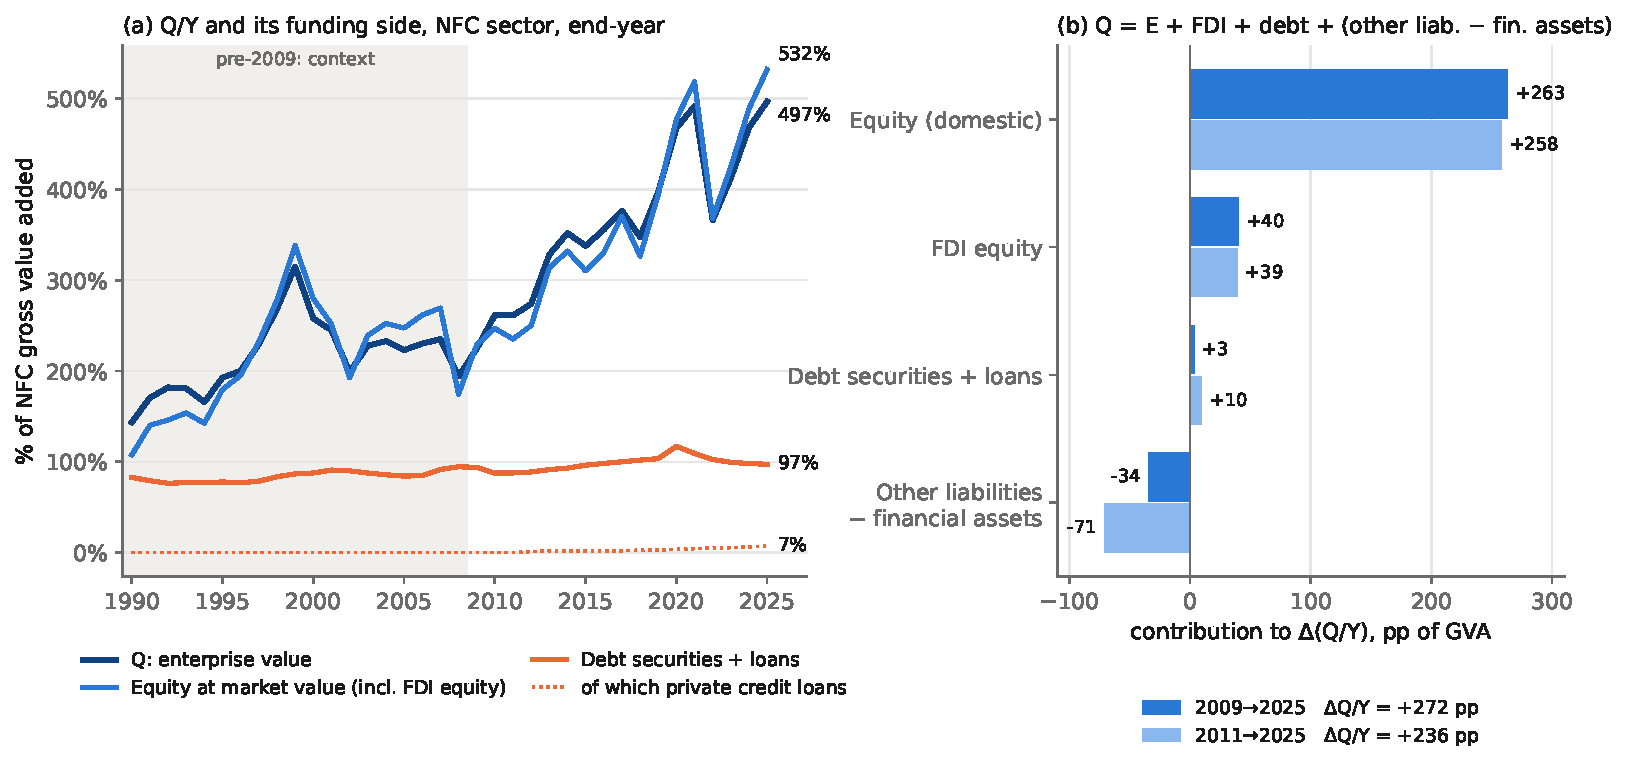
\includegraphics[height=0.47\textheight]{figures/f1_credit_q_funding.pdf}}
\vspace{-0.1cm}
{\scriptsize\setlength{\tabcolsep}{4pt}
\begin{tabular}{@{}lrrrrrr@{}}\toprule
\% of NFC GVA & 2007 & 2009 & 2011 & 2019 & 2025 & \val{latest_q}\\\midrule
Debt securities + loans & \val{DEBTY2007} & \val{DEBTY2009} & \val{DEBTY2011} & \val{DEBTY2019} & \val{DEBTY2025} & \val{lat_DEBTY}\\
\quad bonds / loans & \val{BONDSY2007} / \val{LOANSY2007} & \val{BONDSY2009} / \val{LOANSY2009} & \val{BONDSY2011} / \val{LOANSY2011} & \val{BONDSY2019} / \val{LOANSY2019} & \val{BONDSY2025} / \val{LOANSY2025} & \\
\quad private-credit loans & -- & -- & -- & \val{PCY2019} & \val{PCY2025} & \val{lat_PCY}\\
$Q$ & \val{QY2007} & \val{QY2009} & \val{QY2011} & \val{QY2019} & \val{QY2025} & \val{lat_QY}\\\bottomrule
\end{tabular}}
\src{Z.1 B.103/L.103 via FRED (BCNSDODNS, NCBDBIQ027S, BOGZ1FL103167205Q, NCBEILQ027S, BOGZ1LM103192105Q, TLBSNNCB, TFAABSNNCB, BOGZ1LM102010405Q); GVA BOGZ1FU106902501Q. \val{latest_q}: stocks at end-quarter over trailing four-quarter GVA.}
\end{frame}

% ---------------------------------------------------------------- 5
\begin{frame}{Capital: $K/Y$ is flat; the rise in $Q/Y$ is a rise in Tobin's $q$}{Nonfinancial assets at replacement cost (real estate at market value)}
\centerline{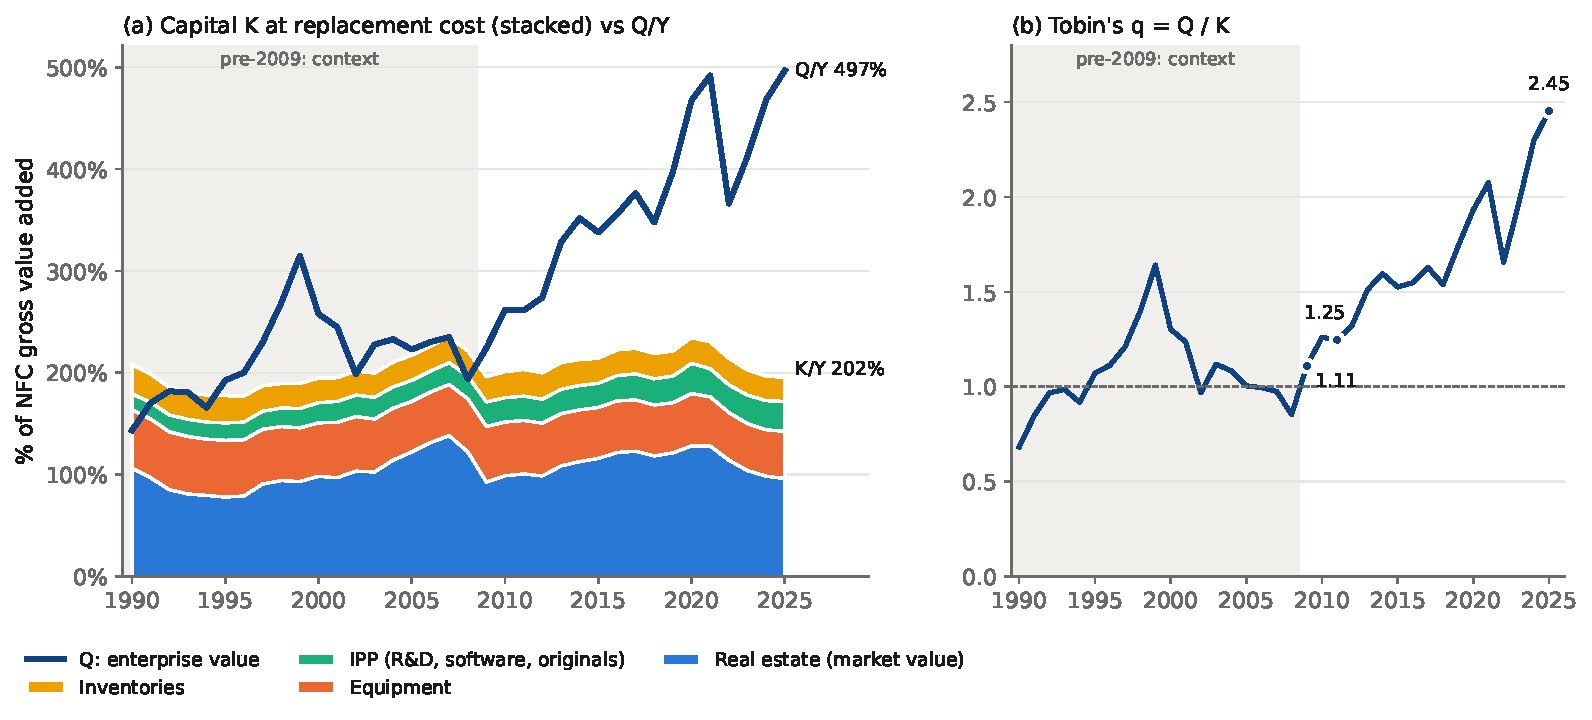
\includegraphics[height=0.47\textheight]{figures/f2_capital_tobin_q.pdf}}
\vspace{-0.1cm}
\begin{columns}[T]
\column{0.5\textwidth}
{\scriptsize\setlength{\tabcolsep}{4pt}
\begin{tabular}{@{}lrrrr@{}}\toprule
 & $\Delta\log\frac{Q}{Y}$ & $=\Delta\log q$ & $+\Delta\log\frac{K}{Y}$ & $q$ share\\\midrule
2009--25 & $\val{dec2009_dlogQY}$ & $\val{dec2009_dlog_q}$ & $\val{dec2009_dlog_KY}$ & \val{dec2009_sh_q}\%\\
2011--25 & $\val{dec2011_dlogQY}$ & $\val{dec2011_dlog_q}$ & $\val{dec2011_dlog_KY}$ & \val{dec2011_sh_q}\%\\\bottomrule
\end{tabular}}
\column{0.46\textwidth}
{\scriptsize Inside $K$, IPP (R\&D, software) rises from \val{IPPY2009}\% to \val{IPPY2025}\% of GVA and equipment falls from \val{EQPY2009}\% to \val{EQPY2025}\%; real estate is \val{REY2009}\% in 2009 and \val{REY2025}\% in 2025, after \val{REY2007}\% at the 2007 peak. $K$ excludes intangibles that the national accounts do not capitalize (organization capital, brands, data), so part of the rise in $q$ may be unmeasured capital rather than price.\par}
\end{columns}
\src{Z.1 B.103: BOGZ1LM102010005Q (total), BOGZ1FL105035023Q + BOGZ1FL105035033Q (real estate), BOGZ1LM105015205Q, BOGZ1LM105013765Q, BOGZ1LM105020015Q.}
\end{frame}

% ---------------------------------------------------------------- 6
\begin{frame}{Flows: internal funds covered net investment}{NFC sector, \% of GVA}
\centerline{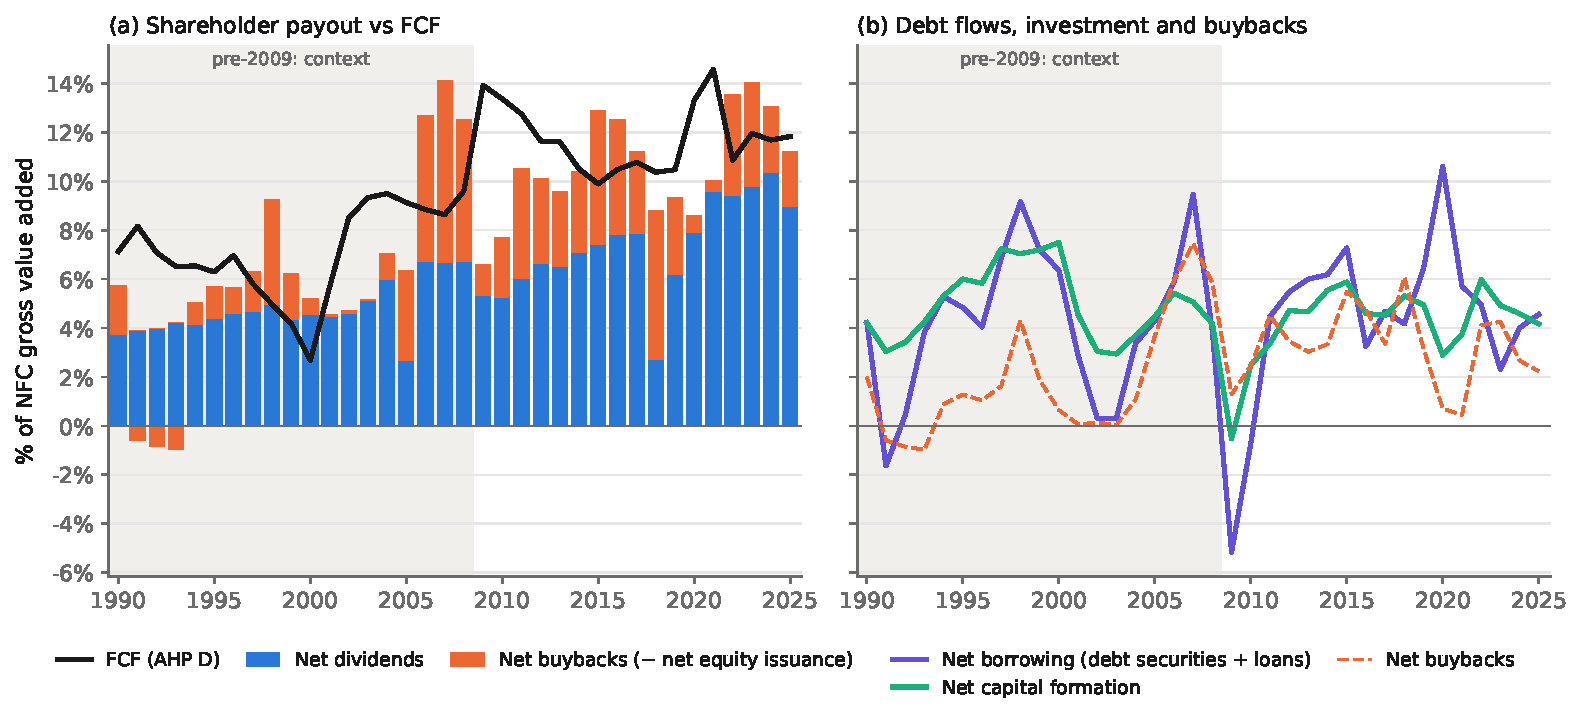
\includegraphics[height=0.47\textheight]{figures/f3_nfc_flows.pdf}}
\vspace{-0.15cm}
\begin{columns}[T]
\column{0.5\textwidth}
{\scriptsize\setlength{\tabcolsep}{4pt}
\begin{tabular}{@{}lrrr@{}}\toprule
Mean, \% of GVA & 1990--2007 & 2009--25 & 2011--25\\\midrule
FCF ($D$) & \val{avg_pre_FCF} & \val{avg_post_FCF} & \val{avg_postB_FCF}\\
Net dividends & \val{avg_pre_DIV} & \val{avg_post_DIV} & \val{avg_postB_DIV}\\
Net buybacks & \val{avg_pre_BUY} & \val{avg_post_BUY} & \val{avg_postB_BUY}\\
Net borrowing & \val{avg_pre_NB} & \val{avg_post_NB} & \val{avg_postB_NB}\\
Net capital formation & \val{avg_pre_NCF} & \val{avg_post_NCF} & \val{avg_postB_NCF}\\\bottomrule
\end{tabular}}
\column{0.46\textwidth}
{\scriptsize Cumulated 2009--25 (tn USD): net borrowing \val{cum_NB}, net capital formation \val{cum_NCF}, net buybacks \val{cum_BUY}, net dividends \val{cum_DIV}. Against this, $Q$ rose by \val{cum_dQ} tn and equity at market value by \val{cum_dEQ} tn. Four quarters to \val{latest_q}: net borrowing \val{lat_NBY}\%, NCF \val{lat_NCFY}\%, net buybacks \val{lat_BUYY}\% (net issuance).\par}
\end{columns}
\src{Z.1 F.103 via FRED: BOGZ1FU104104005Q, BOGZ1FU103164103Q (net buybacks $=-$net equity issuance, includes cash-financed M\&A retirements), BOGZ1FU106121075Q, BOGZ1FU105050985Q; four NSA quarters summed. 2018: TCJA repatriation lowers net dividends.}
\end{frame}

% ---------------------------------------------------------------- 7
\begin{frame}{Where FCF goes: almost all of it to shareholders}{The cash-flow identity of slide 3, NFC sector, Z.1 table S.5.a (closes exactly)}
\centerline{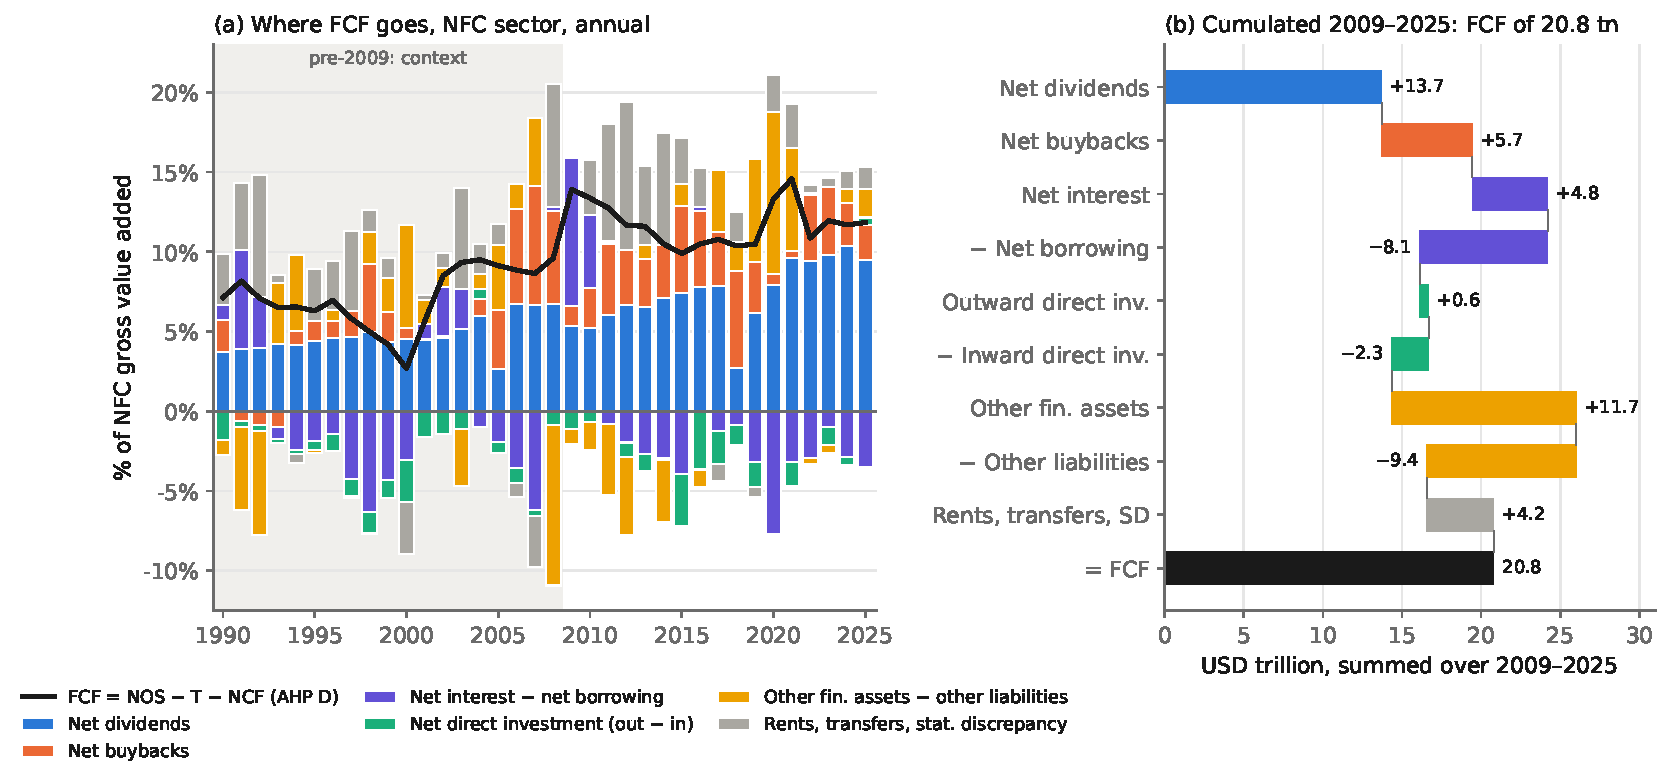
\includegraphics[height=0.47\textheight]{figures/f6_fcf_decomposition.pdf}}
\vspace{-0.15cm}
\begin{columns}[T]
\column{0.55\textwidth}
{\scriptsize\setlength{\tabcolsep}{2.2pt}\renewcommand{\arraystretch}{0.9}
\begin{tabular}{@{}lrrr@{}}\toprule
Mean, \% of GVA & 1990--2007 & 2009--25 & 2011--25\\\midrule
FCF $=\mathrm{NOS}-T-\mathrm{NCF}$ & \val{fd_avg_pre_FCF} & \val{fd_avg_post_FCF} & \val{fd_avg_postB_FCF}\\
\quad Div $+$ BB & \val{fd_avg_pre_DIV} $+$ \val{fd_avg_pre_BUY} & \val{fd_avg_post_DIV} $+$ \val{fd_avg_post_BUY} & \val{fd_avg_postB_DIV} $+$ \val{fd_avg_postB_BUY}\\
\quad Int $-\,\Delta$Debt & \val{fd_avg_pre_INT} $-$ \val{fd_avg_pre_NB} & \val{fd_avg_post_INT} $-$ \val{fd_avg_post_NB} & \val{fd_avg_postB_INT} $-$ \val{fd_avg_postB_NB}\\
\quad Net direct investment & \val{fd_avg_pre_NDI} & \val{fd_avg_post_NDI} & \val{fd_avg_postB_NDI}\\
\quad Other FA $-$ other liab. & \val{fd_avg_pre_NOF} & \val{fd_avg_post_NOF} & \val{fd_avg_postB_NOF}\\
\quad Rent, Tr, KT, SD & \val{fd_avg_pre_OTH} & \val{fd_avg_post_OTH} & \val{fd_avg_postB_OTH}\\\bottomrule
\end{tabular}}
\column{0.42\textwidth}
{\scriptsize 2009--25 (tn USD): $\mathrm{NOS}-T=\val{fd_cuma_NOS_T}$ against $\mathrm{NCF}=\val{fd_cuma_NCF}$, so internal funds alone covered net investment and left FCF $=\val{fd_cuma_FCF}$. Shareholders received \val{fd_cuma_DEQ} (\val{fd_cuma_share_payout}\% of FCF; \val{fd_cumb_share_payout}\% over 2011--25). Creditors put money in on net: borrowing \val{fd_cuma_NB} $>$ interest \val{fd_cuma_INT}. Gross acquisition of financial assets is \val{fd_cuma_NAFA}, but other liabilities rose \val{fd_cuma_OL}: net of them, other financial saving is only \val{fd_cuma_NOF}.\par}
\end{columns}
\src{Z.1 S11.1.i.a (= S.5.a), annual, release of 10 Sep 2026. Div, Int: paid $-$ received. Direct investment: equity flows excluding reinvested earnings (outward $-$ inward). Other liabilities: all except debt securities, loans, corporate equities and FDI equity. Div differs from the FRED net dividends of slide 6 by at most \val{fd_div_diff} tn a year.}
\end{frame}

% ---------------------------------------------------------------- 8
\begin{frame}{Buybacks: payout including buybacks rises with GVA; its yield still falls}{Compustat US nonfinancial firms, and the decomposition with $D$ = shareholder payout}
\centerline{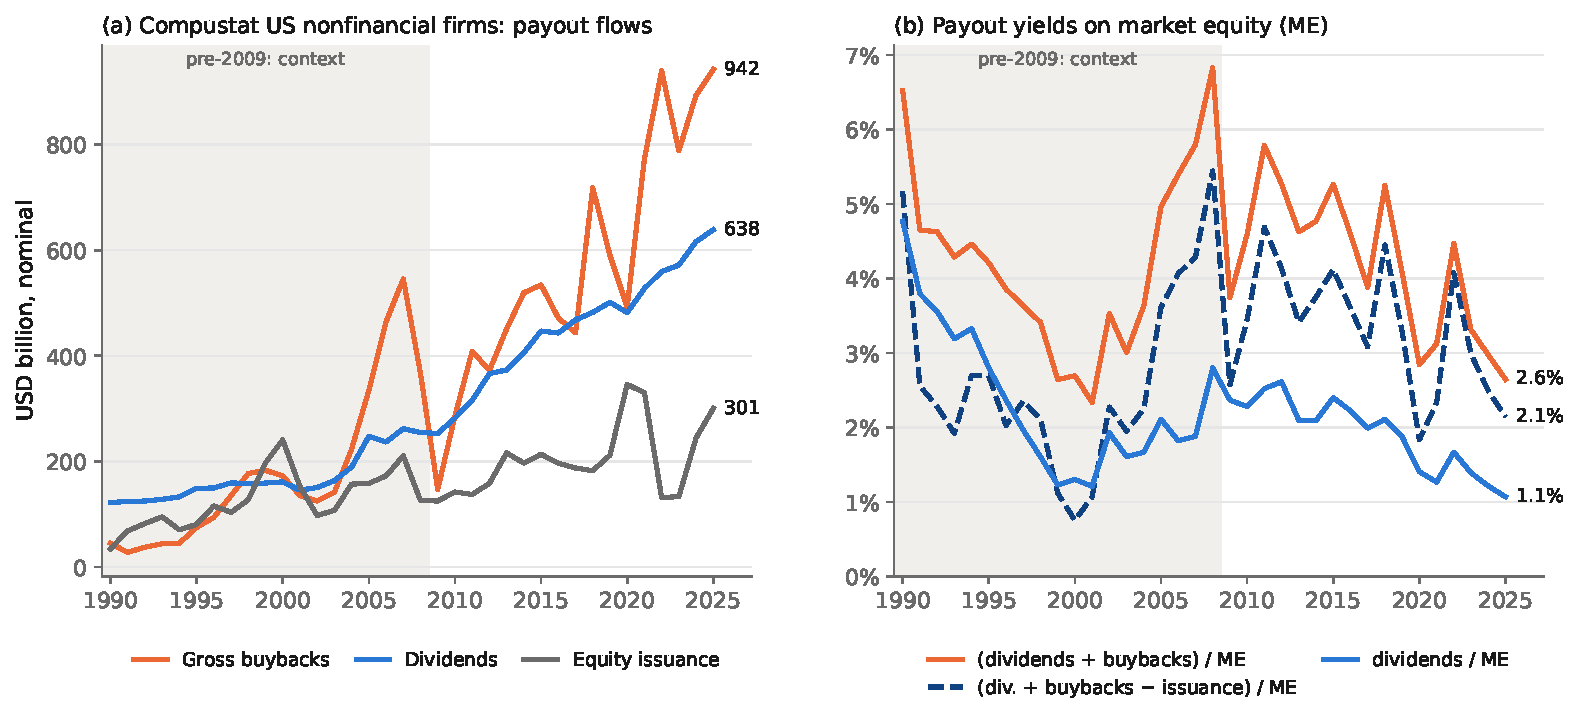
\includegraphics[height=0.47\textheight]{figures/f4_compustat_payout.pdf}}
\vspace{-0.15cm}
\begin{columns}[T]
\column{0.56\textwidth}
{\scriptsize\setlength{\tabcolsep}{3.5pt}
\begin{tabular}{@{}llrrrr@{}}\toprule
Base & $D/Q$, NFC (Z.1) & start & 2025 & $\Delta\log\frac{Q}{Y}$ & $\Delta\log\frac{D}{Y}$\\\midrule
2009 & FCF / $Q$ & \val{rob_fcfa_yield_start}\% & \val{rob_fcfa_yield_end}\% & $\val{rob_fcfa_dlog_QY}$ & $\val{rob_fcfa_dlog_DY}$\\
 & payout / equity & \val{rob_deqa_yield_start}\% & \val{rob_deqa_yield_end}\% & $\val{rob_deqa_dlog_QY}$ & $\val{rob_deqa_dlog_DY}$\\
2011 & FCF / $Q$ & \val{rob_fcfb_yield_start}\% & \val{rob_fcfb_yield_end}\% & $\val{rob_fcfb_dlog_QY}$ & $\val{rob_fcfb_dlog_DY}$\\
 & payout / equity & \val{rob_deqb_yield_start}\% & \val{rob_deqb_yield_end}\% & $\val{rob_deqb_dlog_QY}$ & $\val{rob_deqb_dlog_DY}$\\
3-yr avg & FCF / $Q$ & \val{rob_fcfc_yield_start}\% & \val{rob_fcfc_yield_end}\% & $\val{rob_fcfc_dlog_QY}$ & $\val{rob_fcfc_dlog_DY}$\\
 & payout / equity & \val{rob_deqc_yield_start}\% & \val{rob_deqc_yield_end}\% & $\val{rob_deqc_dlog_QY}$ & $\val{rob_deqc_dlog_DY}$\\\bottomrule
\end{tabular}}
\column{0.4\textwidth}
{\scriptsize Compustat 2009--25: buybacks \$\val{cs_cumbuy} tn, dividends \$\val{cs_cumdiv} tn, issuance \$\val{cs_cumiss} tn; buybacks are \val{cs_buy_share2025}\% of gross payout in 2025. Market equity $\times$\val{cs_me_mult}, gross payout $\times$\val{cs_pay_mult} (2011 base: $\times$\val{cs_me_multB} vs $\times$\val{cs_pay_multB}). Seven AI-related firms are \val{ai7_me_share2009}\% of market equity in 2009, \val{ai7_me_share2025}\% in 2025, and \val{ai7_share_dme}\% of its rise.\par}
\end{columns}
\src{Payout = net dividends + net buybacks; equity = $E+\mathrm{FDI}^{mv}$. 3-yr avg: 2009--11 vs 2023--25. Compustat funda, fic = USA, SIC outside 6000--6999; ME = csho$\times$prcc\_f. AI-related seven: AAPL, MSFT, GOOGL, AMZN, META, NVDA, ORCL.}
\end{frame}

% ---------------------------------------------------------------- 9
\begin{frame}{Where firm borrowing went: a range, not a point}{Compustat US nonfinancial firms: positive net borrowing split by use inside each firm-year}
\centerline{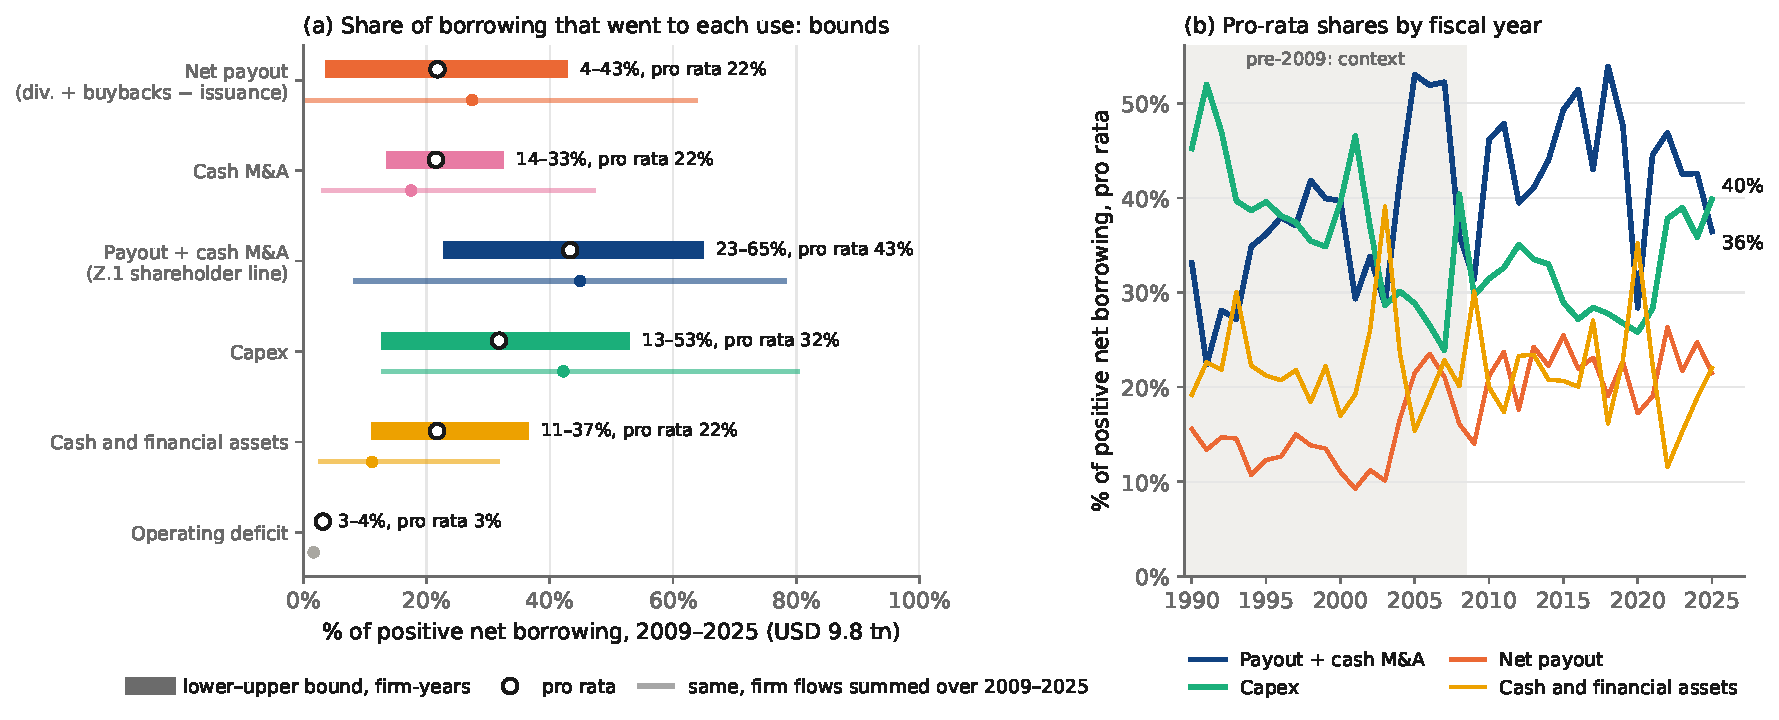
\includegraphics[height=0.47\textheight]{figures/f7_debt_use_bounds.pdf}}
\vspace{-0.15cm}
\begin{columns}[T]
\column{0.5\textwidth}
{\scriptsize \textbf{How the bounds work.} Each firm-year: OCF $+$ net borrowing $=$ capex $+$ cash M\&A $+$ net payout $+$ cash and other financial uses. Money is fungible inside a firm, so a use's share of the borrowing is only bounded: \emph{lower} if internal funds pay that use first, \emph{upper} if they pay it last; \emph{pro rata} splits the borrowing in proportion to the uses. Firms with positive net borrowing raised \$\val{du_ndp} tn in 2009--25; the others repaid \$\val{du_ndm} tn (net \$\val{du_nd_net} tn; Z.1 NFC \$\val{cum_NB} tn).\par}
\column{0.46\textwidth}
{\scriptsize \textbf{What is robust.} Only \val{du_PAY_lo}\% of the borrowing must have paid shareholders, against \val{du_INV_lo}\% for capex and \val{du_MA_lo}\% for cash M\&A. Pro rata, payout + cash M\&A (the Z.1 shareholder line) takes \val{du_PAYMA_pr}\% and capex \val{du_INV_pr}\%, but the ranges overlap. Debt paid \val{du_paydebt_lo}--\val{du_paydebt_hi}\% of payouts (\val{du_paydebt_pr}\% pro rata). Capex's pro-rata share: \val{du_inv_pr_min_pre}--\val{du_inv_pr_max_pre}\% a year to 2021, \val{du_inv_pr_min_ai}--\val{du_inv_pr_max_ai}\% in 2022--25.\par}
\end{columns}
\src{Compustat funda as on slide 8, oancf reported: \val{du_nfy} firm-years, \val{du_nfirms} firms. Net borrowing $=$ dltis $-$ dltr $+$ dlcch; net payout $=$ dvt $+$ prstkc $-$ sstk; cash M\&A $=$ aqc; cash and other is the residual. Gross payout: payout \val{dug_PAY_lo}--\val{dug_PAY_hi}\%; R\&D as investment: capex $+$ R\&D \val{dur_INV_lo}--\val{dur_INV_hi}\%. Global consolidated firms; Z.1 is domestic.}
\end{frame}

% ---------------------------------------------------------------- 10
\begin{frame}{The AI cycle: debt-financed capex since late 2025}{MSFT, GOOGL, AMZN, META, ORCL (and CoreWeave), Compustat quarterly}
\centerline{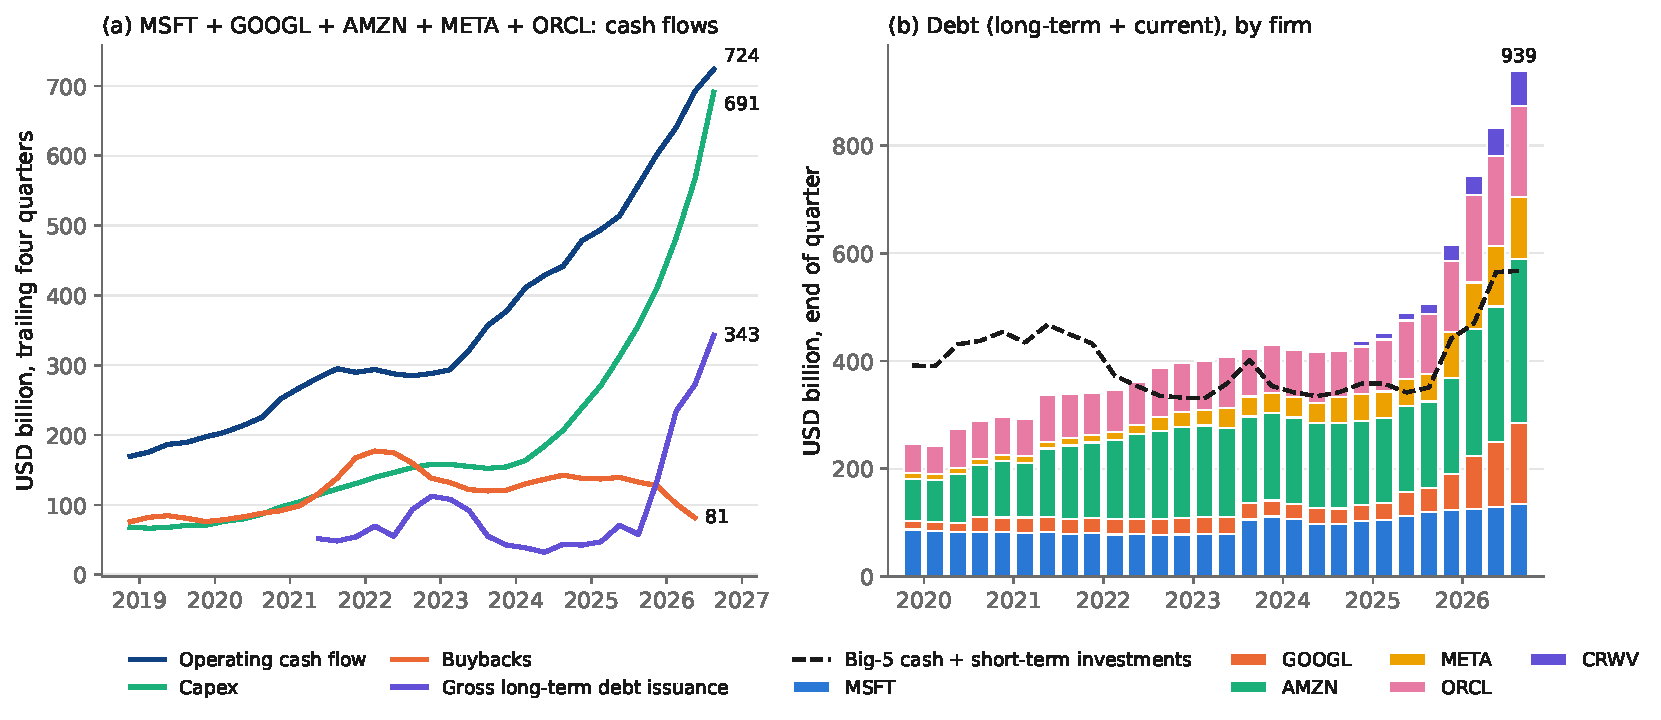
\includegraphics[height=0.47\textheight]{figures/f5_ai_hyperscalers.pdf}}
\vspace{-0.1cm}
\begin{columns}[T]
\column{0.5\textwidth}
{\scriptsize\setlength{\tabcolsep}{4pt}
\begin{tabular}{@{}lrrrr@{}}\toprule
Big five, USD bn & 2019Q4 & 2023Q4 & 2025Q4 & \val{ai_last_q}\\\midrule
Capex, trailing 4Q & \val{b5_capx_2019q4} & \val{b5_capx_2023q4} & \val{b5_capx_2025q4} & \val{b5_capx_2026q3}\\
Operating cash flow, 4Q & \val{b5_oancf_2019q4} & \val{b5_oancf_2023q4} & \val{b5_oancf_2025q4} & \val{b5_oancf_2026q3}\\
Capex / OCF & \val{b5_ratio_2019q4}\% & \val{b5_ratio_2023q4}\% & \val{b5_ratio_2025q4}\% & \val{b5_ratio_2026q3}\%\\
Debt, end of quarter & \val{b5_debt_2019q4} & \val{b5_debt_2023q4} & \val{b5_debt_2025q4} & \val{b5_debt_2026q3}\\\bottomrule
\end{tabular}}
\column{0.46\textwidth}
{\scriptsize Until 2024 capex was paid out of operating cash flow and buybacks continued. Since 2025Q4: gross long-term debt issuance \$\val{b5_dltis_2026q3}bn over four quarters (net \$\val{b5_netiss_2026q3}bn), buybacks down to \$\val{b5_buy_2026q2}bn (to \val{ai_last_qbuy}). CoreWeave debt \$\val{crwv_debt_last}bn. Off-balance-sheet data-center financing (joint ventures, leases not yet commenced) is not in these numbers.\par}
\end{columns}
\src{Compustat fundq; flows from fiscal year-to-date items; quarters mapped to calendar quarters by datadate (ORCL ends one month earlier). Debt = dlttq + dlcq; cash = cheq. Global consolidated firms; Z.1 NFC is domestic, so the shares on slide 2 are orders of magnitude.}
\end{frame}

% ---------------------------------------------------------------- 11
\begin{frame}{What this means for the model}
\vspace{0.15cm}
\begin{columns}[T]
\column{0.48\textwidth}
{\small
\textbf{What the data rule out for 2009--2025}
\begin{itemize}\setlength{\itemsep}{0.12cm}
\item A credit channel: NFC debt/GVA is flat, internal funds alone covered net investment, and \val{fd_cuma_share_payout}\% of FCF went to shareholders.
\item A measured-capital channel: $K/Y$ is flat, so $Q/Y$ rises only through $q=Q/K$.
\item A buyback reading of the yield fall: including buybacks raises $D/Y$.
\end{itemize}}
\column{0.48\textwidth}
{\small
\textbf{What is left}
\begin{itemize}\setlength{\itemsep}{0.12cm}
\item A rise in $q$: the price of claims over replacement cost, concentrated in a few large firms (\val{ai7_share_dme}\% of the rise in market equity). Candidates: rents, unmeasured intangibles, or a lower required return (the funding side of the 16 Nov deck).
\item The AI cycle (2025--26) is the first episode in the window where capex and debt rise together; it can be tracked quarter by quarter in Z.1 and Compustat.
\end{itemize}}
\end{columns}
\vfill
{\small\textcolor{inksec}{Next data, if useful: Z.1 2026Q3 (December 2026) for the NFC aggregates; gross bond issuance by issuer (SIFMA, or Mergent FISD on WRDS) to separate AI issuers; S\&P 500 buyback series (S\&P Dow Jones Indices) as a third buyback source; stated use of proceeds for bonds (Capital IQ Transactions or LSEG Workspace; DealScan already gives loan purposes).}}
\vspace{0.4cm}
\end{frame}

% ---------------------------------------------------------------- 12-14: slide 3 explained, for readers new to these data
\begin{frame}[label=xvalue]{Appendix: the value side of slide 3, explained}{What $Q$ measures, and why it is split by type of claim}
\vspace{-0.15cm}
\begin{columns}[T]
\column{0.47\textwidth}
{\scriptsize\textbf{Market-value balance sheet, NFC, end-2025 (USD tn)}\\[0.08cm]
\setlength{\tabcolsep}{2pt}
\begin{tabular}{@{}lr|lr@{}}\toprule
\multicolumn{2}{@{}l|}{\textbf{What firms own}} & \multicolumn{2}{l@{}}{\textbf{Claims on firms}}\\\midrule
\textcolor{dataD}{\textbf{Nonfinancial assets $Q$}} & \textcolor{dataD}{\textbf{\val{bs2025_Q}}} & Equity $E$ & \val{bs2025_E}\\
\quad\textcolor{inksec}{(backed out)} & & Foreign parents, FDI$^{mv}$ & \val{bs2025_FDI}\\
Financial assets FA & \val{bs2025_FA} & Debt & \val{bs2025_DEBT}\\
 & & Other liabilities OL & \val{bs2025_OL}\\\midrule
Total & \val{bs2025_TOT} & Total & \val{bs2025_TOT}\\\bottomrule
\end{tabular}\\[0.12cm]
Market prices exist for the claims on the right, not for the factories, software and brands on the left. Z.1 therefore backs $Q$ out of the two totals:
\[Q=E+\mathrm{FDI}^{mv}+\mathrm{Debt}+\mathrm{OL}-\mathrm{FA}.\]
\textcolor{inksec}{FDI$^{mv}$: equity of foreign parents in their US affiliates. FA: cash and deposits, receivables, securities, US firms' equity in their foreign affiliates. OL: trade and tax payables, pension liabilities, intercompany debt owed to foreign parents.}\par}
\column{0.49\textwidth}
{\scriptsize
\begin{itemize}\setlength{\itemsep}{0.07cm}
\item \textbf{What $Q$ is.} The price of the whole business: buy every share, take over every debt and payable, keep the cash and other financial assets.
\item \textbf{Why it is the model's $Q$.} In the model the firm has one claim, worth the present value of future $D$. In the data the cash flows are shared by shareholders, creditors and others; the sum of all claims does not depend on how the firm is financed.
\item \textbf{Why FA is netted out.} Cash and securities are not productive capital; foreign affiliates are not US capital. A firm that borrows to hold cash raises Debt and FA together, and $Q$ does not move.
\item \textbf{Why split by claim.} Divided by $Y$, the terms add up to $Q/Y$, so a change in $Q/Y$ splits exactly by claim: credit shows up in Debt$/Y$, equity (issued or revalued) in $E/Y$. 2009$\to$2025, pp of GVA (slide 4): $Q/Y$ $+\val{dec2009_dQY_pp}$ $=$ $E$ $+\val{dec2009_dEY_pp}$, FDI$^{mv}$ $+\val{dec2009_dFDIY_pp}$, Debt $+\val{dec2009_dDEBTY_pp}$, OL$-$FA $\val{dec2009_dOTHERY_pp}$.
\item \textbf{What it cannot say.} A debt-financed buyback swaps $E$ for Debt one for one, so the split shows which claims grew, not why. Telling new money from price changes needs the flows (slide \hyperlink{xlink}{14}).
\end{itemize}}
\end{columns}
\src{Z.1 B.103/L.103 via FRED, as on slides 3--4; the identity is the Fed's definition of FL102010405 (market value estimate of nonfinancial assets). Unlisted firms' equity is not traded; its market value is a Fed estimate.}
\end{frame}

\begin{frame}[label=xcash]{Appendix: the cash-flow side of slide 3, explained}{What FCF measures, and why it is split by who receives it}
\vspace{-0.15cm}
\begin{columns}[T]
\column{0.41\textwidth}
{\scriptsize\textbf{Worked example: one firm, one year}\\[0.05cm]
Operating surplus after wages, production taxes and depreciation (NOS) 100; income tax 20; net investment 30; interest 5. So $\mathrm{FCF}=100-20-30=50$, whatever the firm does next:\\[0.08cm]
\setlength{\tabcolsep}{4pt}
\begin{tabular}{@{}lrrrr@{}}\toprule
 & (a) & (b) & (c) & (d)\\\midrule
Dividends & 45 & 0 & 45 & 25\\
Buybacks & 0 & 45 & 20 & 0\\
Interest & 5 & 5 & 5 & 5\\
$-$ New borrowing & 0 & 0 & $-20$ & 0\\
Kept as cash & 0 & 0 & 0 & 20\\\midrule
$=$ FCF & 50 & 50 & 50 & 50\\\midrule
To shareholders & 45 & 45 & 65 & 25\\
To creditors & 5 & 5 & $-15$ & 5\\\bottomrule
\end{tabular}\\[0.08cm]
(a) pays dividends; (b) buys back shares instead; (c) also borrows 20 to buy back more; (d) keeps 20 as cash. Dividends alone would fall to 0 in (b), with nothing changed in the business.\par}
\column{0.55\textwidth}
{\scriptsize
\begin{itemize}\setlength{\itemsep}{0.07cm}
\item \textbf{What FCF is.} Cash left after wages, taxes, depreciation and net investment (NCF), before any payment to shareholders or creditors.
\item \textbf{Why it is the model's $D$.} $D$ must be the cash flow of the claims that $Q$ values: all claims, net of financial assets. So $D$ is all payments to them, net of new borrowing and of cash kept: FCF.
\item \textbf{Why not dividends.} US payout has shifted from dividends to buybacks since the 1980s. Dividends alone would show a fall that is only a change of form (column b).
\item \textbf{Why split by recipient.} Does payout form matter (shareholder line)? Did borrowing pay for payouts (sign of the creditor line)? Do firms hoard cash (net financial saving)? 2009--25: \val{fd_cuma_share_payout}\% of FCF went to shareholders (slide 7).
\item \textbf{Why it closes exactly.} Income not taxed or invested is paid out or changes financial assets or liabilities. Income data are from BEA, financial data from the Fed; SD is the gap. The identity always holds; the content is in the size of each term.
\item \textbf{What it cannot say.} Money is fungible: the split says how much went to each group, not which source paid for which use. A cash takeover of one US firm by another is a buyback for the sector.
\end{itemize}}
\end{columns}
\src{In the data, ``kept as cash'' is net financial saving, NAFA $-\,\Delta$OL $-$ RE (slide 3): purchases of all financial assets, net of other new liabilities and of foreign affiliates' reinvested earnings (income earned abroad, so not in NOS). Rent, Tr, KT and SD are the remaining small items (glossary, slide 16). Which firm's borrowing paid for which use: slide 9.}
\end{frame}

\begin{frame}[label=xlink]{Appendix: how the two sides connect}{Change in a stock $=$ net transactions (the cash-flow side) $+$ revaluation; NFC sector, USD tn}
\vspace{-0.15cm}
\begin{columns}[T]
\column{0.52\textwidth}
{\scriptsize\setlength{\tabcolsep}{3pt}\textbf{End-2009 to end-2025}\\[0.05cm]
\begin{tabular}{@{}lrrrr@{}}\toprule
 & Change & $=$ Net & $+$ Reval- & $+$ Other\\
 & in stock & transactions & uation & changes\\\midrule
Equity, $E$ & $\val{sf2009_E_change}$ & $\val{sf2009_E_flows}$ & $\val{sf2009_E_reval}$ & $\val{sf2009_E_other}$\\
FDI$^{mv}$ & $\val{sf2009_FDI_change}$ & $\val{sf2009_FDI_flows}$ & $\val{sf2009_FDI_reval}$ & $\val{sf2009_FDI_other}$\\
Debt & $\val{sf2009_DEBT_change}$ & $\val{sf2009_DEBT_flows}$ & -- & $\val{sf2009_DEBT_other}$\\
Other liabilities, OL & $\val{sf2009_OL_change}$ & $\val{sf2009_OL_flows}$ & $\val{sf2009_OL_reval}$ & $\val{sf2009_OL_other}$\\
$-$ Financial assets, FA & $\val{sf2009_MFA_change}$ & $\val{sf2009_MFA_flows}$ & $\val{sf2009_MFA_reval}$ & $\val{sf2009_MFA_other}$\\\midrule
$=Q$ & $\mathbf{\val{sf2009_Q_change}}$ & $\mathbf{\val{sf2009_Q_flows}}$ & $\mathbf{\val{sf2009_Q_reval}}$ & $\val{sf2009_Q_other}$\\\bottomrule
\end{tabular}\\[0.1cm]
\textcolor{inksec}{Net transactions are the flows of the cash-flow side: new shares minus shares retired ($-$BB), net borrowing, purchases of financial assets (NAFA). Revaluation is the change in the value of a stock that is not a transaction: holding gains and losses (Fed revaluation account). Debt is at book value, so it has none. Other changes: reclassifications, write-offs and breaks in the source data.}\par}
\column{0.44\textwidth}
{\scriptsize
\begin{itemize}\setlength{\itemsep}{0.1cm}
\item \textbf{Equity.} Firms retired a net \$\val{sf2009_E_flows_abs} tn of their own shares, yet the market value of their equity rose \$\val{sf2009_E_change} tn. None of the rise came from new shares.
\item \textbf{All claims.} $Q$ rose \$\val{sf2009_Q_change} tn. Net new money from all claim holders, net of financial assets bought, was \$\val{sf2009_Q_flows} tn: \val{sf2009_Q_reval_share}\% of the rise is revaluation (\val{sf2011_Q_reval_share}\% from end-2011).
\item \textbf{What revaluation contains.} The value of investment paid for out of retained earnings (no new claims are issued for it) and price changes. The capital side separates the two: $K$ at replacement cost rose \$\val{sf2009_dK} tn, so most of the rise in $Q$ is a rise in $q=Q/K$ (slide 5).
\item \textbf{Why both sides.} The value side alone cannot tell new claims from higher prices; the cash-flow side alone says nothing about prices.
\end{itemize}}
\end{columns}
\src{Z.1 S11.1.i.a (= S.5.a): levels, transactions (FU) and revaluations (FR) from one table; other changes $=$ change $-$ transactions $-$ revaluation. Stocks at end-2009 and end-2025, so flows are summed over 2010--25 (slide 7 sums 2009--25). Rounded to 0.1. From end-2011: $Q$ $+$\val{sf2011_Q_change}, transactions $+$\val{sf2011_Q_flows}, revaluation $+$\val{sf2011_Q_reval}.}
\end{frame}

% ---------------------------------------------------------------- 15
\begin{frame}{Appendix: sources and rebuild}
\vspace{0.1cm}
{\scriptsize
\textbf{Z.1 / NIPA via FRED} (retrieved 2026-11-18, data through \val{latest_q}): 30 series, listed with titles and units in data/raw/fred/\_metadata.csv. Annual flows are sums of four NSA quarters; stocks are end of Q4.\\[0.12cm]
\textbf{Z.1 table S11.1.i.a (= S.5.a)} (Fed CSV release of 10 Sep 2026, retrieved 2026-11-18): annual NFC integrated accounts for the FCF decomposition; data/raw/fed\_z1 with the line dictionary and manifest.json.\\[0.12cm]
\textbf{Compustat} (WRDS, retrieved 2026-11-18): comp.funda for US-incorporated USD filers, fiscal 1989--2026 (2026 incomplete, not used); comp.fundq for AAPL, MSFT, ORCL, CRWV, AMZN, NVDA, GOOGL, META from 2014. Manifest in data/raw/wrds/manifest.json. Licensed data: not for redistribution.\\[0.12cm]
\textbf{Processed data}: data/processed (z1\_nfc\_annual\_trn.csv, z1\_nfc\_ratios\_pct\_gva.csv, z1\_q\_decomposition.csv, fcf\_decomposition\_nfc\_trn.csv, fcf\_decomposition\_nfc\_pct\_gva.csv, stock\_flow\_reconciliation\_nfc\_trn.csv, payout\_robustness\_nfc.csv, compustat\_nonfin\_annual\_bn.csv, debt\_use\_bounds\_annual.csv, debt\_use\_bounds\_summary.csv, ai\_big5\_quarterly\_bn.csv, ai\_firms\_debt\_by\_firm\_bn.csv, ai\_firms\_quarterly\_musd.csv).\\[0.12cm]
\textbf{Definitions.} Net buybacks $=-$Z.1 net equity issuance (net of IPOs and issuance, includes cash M\&A retirements). Compustat buybacks are gross (prstkc: common and preferred). NFC $D=\mathrm{NOS}-T-\mathrm{NCF}$, the AHP FCF for the NFC sector.\\[0.12cm]
\textbf{Rebuild.} \texttt{cd scripts}; \texttt{uv run --no-project --python 3.12 python -I fetch\_fred.py}; the same for fetch\_z1.py; WRDS pull with fetch\_wrds.py (see its header); debt\_use\_bounds.py (same uv line, without matplotlib); \texttt{uv run --no-project --python 3.12 --with numpy==2.3.5 --with pandas==2.2.3 --with matplotlib==3.10.0 python -I build.py}; then \texttt{latexmk -pdf credit\_capital\_buybacks\_2026\_11\_18.tex} in the folder.}
\end{frame}

% ---------------------------------------------------------------- 16-17
\newcommand{\gl}[2]{\textbf{#1} & #2\\}
\begin{frame}{Appendix: abbreviations and symbols (1/2)}{Accounting terms; NFC sector unless stated; flows are annual transactions, stocks end of year}
\vspace{-0.05cm}
\begin{columns}[T]
\column{0.49\textwidth}
{\tiny\setlength{\tabcolsep}{3pt}\renewcommand{\arraystretch}{1.12}
\begin{tabular}{@{}>{\raggedright}p{0.17\linewidth}p{0.79\linewidth}@{}}\toprule
\gl{NFC}{Nonfinancial corporate business, the Z.1 sector used throughout}
\gl{$Y$, GVA}{Gross value added of the NFC sector}
\gl{$Q$}{Enterprise value: market value of NFC nonfinancial assets (Z.1 FL102010405) $=E+\mathrm{FDI}^{mv}+\mathrm{TL}-\mathrm{FA}$; the AHP $Q$}
\gl{$E$}{Corporate equities issued by NFCs, market value}
\gl{FDI$^{mv}$}{Foreign direct investment in the US (equity in US affiliates of foreign parents), market value}
\gl{TL, FA}{Total liabilities (excluding equity); total financial assets}
\gl{Debt}{Debt securities (corporate bonds, commercial paper, municipal) $+$ loans (bank, private credit, mortgages, other)}
\gl{OL}{Other liabilities $=\mathrm{TL}-\mathrm{Debt}$: trade payables, taxes payable, pension entitlements, FDI intercompany debt, miscellaneous}
\gl{$K$}{Nonfinancial assets at replacement cost: real estate at market value; equipment, IPP and inventories at current cost}
\gl{$q$}{Tobin's $q=Q/K$}
\gl{IPP}{Intellectual property products: R\&D, software, entertainment and artistic originals}
\gl{$D$, FCF}{Free cash flow $=\mathrm{NOS}-T-\mathrm{NCF}$, the AHP dividend measure}
\gl{NOS}{Net operating surplus: GVA $-$ compensation of employees $-$ taxes on production and imports (less subsidies) $-$ consumption of fixed capital}\bottomrule
\end{tabular}}
\column{0.49\textwidth}
{\tiny\setlength{\tabcolsep}{3pt}\renewcommand{\arraystretch}{1.12}
\begin{tabular}{@{}>{\raggedright}p{0.17\linewidth}p{0.79\linewidth}@{}}\toprule
\gl{$T$}{Current taxes on corporate income, wealth, etc.}
\gl{NCF}{Net capital formation: gross fixed investment $+$ inventory change $+$ net purchases of nonproduced assets $-$ consumption of fixed capital}
\gl{Div}{Net dividends: dividends paid $-$ dividends received}
\gl{BB}{Net buybacks $=-$ net issuance of corporate equities (net of IPOs and new issues; includes shares retired in cash M\&A)}
\gl{Int}{Net interest: interest paid $-$ interest received}
\gl{$\Delta$Debt, NB}{Net borrowing: net incurrence of debt securities and loans}
\gl{NAFA}{Net acquisition of financial assets}
\gl{$\Delta$OL}{Net incurrence of OL, plus inward FDI equity flows}
\gl{RE}{Reinvested earnings on direct investment, net: earned by US firms' foreign affiliates $-$ earned by foreign parents on US affiliates. Recorded as income and as a direct-investment flow, but not in NOS}
\gl{Net direct inv.}{Outward direct-investment equity flow $-$ inward FDI equity flow, both excluding reinvested earnings}
\gl{Rent}{Rents paid on land and natural resources}
\gl{Tr}{Other current transfers paid (e.g.\ legal settlements, donations)}
\gl{KT}{Net capital transfers paid}
\gl{SD}{Statistical discrepancy of the NFC accounts (capital-account minus financial-account net lending)}\bottomrule
\end{tabular}}
\end{columns}
\end{frame}

\begin{frame}{Appendix: abbreviations and symbols (2/2)}{Models, data sources, firm-level items and other shorthand}
\vspace{-0.05cm}
\begin{columns}[T]
\column{0.49\textwidth}
{\tiny\setlength{\tabcolsep}{3pt}\renewcommand{\arraystretch}{1.12}
\begin{tabular}{@{}>{\raggedright}p{0.17\linewidth}p{0.79\linewidth}@{}}\toprule
\gl{HKT}{Hirano, Kishi and Toda, \emph{Technological innovation and bursting bubbles}; the project's model}
\gl{AHP}{Atkeson, Heathcote and Perri; source of the $Q$ (enterprise value) and $D$ (FCF) mappings from Z.1}
\gl{MM}{Modigliani--Miller: financing and payout form do not change firm value or FCF}
\gl{Z.1}{Financial Accounts of the United States (Federal Reserve)}
\gl{B.103, L.103, F.103}{Z.1 tables for the NFC sector: balance sheet, liabilities and assets (levels), flows}
\gl{S.5.a (S11.1.i.a)}{Z.1 integrated macroeconomic accounts for the NFC sector, annual (new table name in brackets)}
\gl{IMA}{Integrated macroeconomic accounts (Fed--BEA)}
\gl{NIPA, BEA}{National Income and Product Accounts; Bureau of Economic Analysis}
\gl{FRED}{Federal Reserve Economic Data (St.\ Louis Fed), used to download Z.1 series}
\gl{FL, FU, LM, FR}{Z.1 series prefixes: level, unadjusted flow (transactions), market-value level, revaluation}
\gl{NSA}{Not seasonally adjusted}
\gl{TTM, 4Q}{Trailing twelve months: sum of the last four quarters}
\gl{pp}{Percentage points}
\gl{Lower, upper, pro rata}{Slide 9: share of a firm's positive net borrowing that went to a use if internal funds pay that use first, last, or in proportion to the uses}
\gl{tn, bn}{Trillion, billion (USD, nominal)}\bottomrule
\end{tabular}}
\column{0.49\textwidth}
{\tiny\setlength{\tabcolsep}{3pt}\renewcommand{\arraystretch}{1.12}
\begin{tabular}{@{}>{\raggedright}p{0.17\linewidth}p{0.79\linewidth}@{}}\toprule
\gl{WRDS}{Wharton Research Data Services}
\gl{Compustat}{S\&P firm accounts: funda (annual), fundq (quarterly)}
\gl{prstkc}{Purchase of common and preferred stock (gross buybacks)}
\gl{sstk, dvt}{Sale of common and preferred stock (issuance); total dividends}
\gl{dltt, dlc}{Long-term debt; debt in current liabilities}
\gl{dltis, dltr, dlcch}{Long-term debt issuance; long-term debt reduction; change in current debt}
\gl{che, oancf, capx, aqc}{Cash and short-term investments; operating cash flow (OCF); capital expenditure (capex); acquisitions (cash M\&A)}
\gl{ME}{Market equity $=$ shares outstanding (csho) $\times$ fiscal-year-end price (prcc\_f)}
\gl{SIC}{Standard Industrial Classification; 6000--6999 (finance) excluded}
\gl{Big five}{AI hyperscalers MSFT (Microsoft), GOOGL (Alphabet), AMZN (Amazon), META (Meta), ORCL (Oracle)}
\gl{AI-related seven}{Big five $+$ AAPL (Apple), NVDA (Nvidia)}
\gl{CRWV}{CoreWeave}
\gl{TCJA}{Tax Cuts and Jobs Act (2017), which triggered the 2018 repatriation of foreign earnings}
\gl{M\&A, IPO}{Mergers and acquisitions; initial public offering}\bottomrule
\end{tabular}}
\end{columns}
\end{frame}

\end{document}
